\documentclass[oneside,12pt]{Classes/VTU}
\title{Prediction of heart disease and diabetes using machine learning}
\author{by \\ \vspace{1mm}
\begin{tabular}{ccc}
\textbf{Akshat Agarwal }&  & \textbf{1SI16CS010}\\
\textbf{Akarsh Singh }&  & \textbf{1SI16CS007}\\
\textbf{Ayush Bhargava }&  & \textbf{1SI16CS131}\\
\textbf{Srijan Yadav }&  & \textbf{1SI16CS109}\\
\end{tabular}
\vspace{7mm} \\under the guidance of\\\textbf{H.K Vedamurthy}
\\Assistant Professor \vspace{0.5cm}}
%for Associate Professor - Associate Professor
%for Professor - Professor

\collegeordept{Department of Computer Science and Engineering}
\university{Siddaganga Institute of Technology, Tumakuru}

\renewcommand{\submittedtext}{A project report submitted to \\Visvesvaraya Technological University. Belgaum, Karnataka \\\textit{in the partial fulfillment of the requirements for the award of degree of} }
\degree{\textbf{\textit{Bachelor of Engineering}} \\ in \\ \textbf{\textit{Computer Science and Engineering}}}
\degreedate{\textbf{May, 2020}}

\hbadness=10000
\hfuzz=50pt

\usepackage[inner=1.2in, outer=1in, top=1.2in, bottom=1.2in]{geometry}

\date{2020}

%\setcounter{tocdepth}{3}
%\setcounter{secnumdepth}{3}

%%% Landscape
\usepackage{pdflscape}

%%% Content in multiple columns
\usepackage{multicol}

%%% Colors
\usepackage[dvipsnames]{xcolor}

%%% Text Spacing
\usepackage{setspace}

%%% Maths
\usepackage{amsmath}

%%% Packages for tables
\usepackage{arydshln}
\usepackage{multirow}
\renewcommand{\arraystretch}{1.5}

%Packages for Figures
\usepackage{graphicx}
\setlength{\fboxrule}{2pt}

%Packages for Subfigures
\usepackage{caption}
\usepackage{subcaption}

\usepackage{StyleFiles/watermark}
\usepackage{multirow}
\usepackage{epsfig}
\usepackage{enumerate}
\usepackage{amsmath}
\usepackage{amsthm}
\usepackage{amscd}
\usepackage{amssymb}
\usepackage{rotating}
\usepackage{graphicx}
\usepackage{algorithm}
\usepackage{algorithmic}
\usepackage{setspace}
\usepackage[T1]{fontenc}
\usepackage{alltt}
\usepackage{array}

\usepackage{float}

\begin{document}

\renewcommand\baselinestretch{1.2}
\baselineskip=18pt plus1pt

\maketitle

\setcounter{tocdepth}{3}
\setcounter{secnumdepth}{3}
	
\begin{romanpages}
\begin{center}
\bfseries
\large{Department of Computer Science and Engineering\\
Siddaganga Institute of Technology \\
Tumakuru - 572103} \\
\begin{figure}[hbtp]
\centering

\includegraphics[scale=1]{../ThesisFigs/College_logo.png}
\end{figure}

\LARGE{CERTIFICATE} \\
\end{center}
\small{
Certified that the Project Report entitled \textbf{"Prediction of Heart disease and diabetes using machine learning"} is a bonafide work carried out by \textbf{Akshat Agarwal (1SI16CS010), Akarsh Singh (1SI16CS007), Ayush Bhargava (1SI16CS131) and Srijan Yadav (1SI16CS109)} in the partial fulfillment of the requirement for the award of the degree of Bachelor of Engineering in Computer Science and Engineering , Visvesvaraya Technological University, Belagavi during the year 2015-16. It is certified that all corrections/suggestions indicated for the internal assessment have been incorporated in the report. The project report has been approved as it satisfies the academic requirements in respect of project work prescribed for the Bachelor of Engineering Degree.} \\

\begin{table}[h!]
\centering
\begin{tabular}{cccccccccc}
.................................&&&&&&&&& .................................\\
\textbf{{\footnotesize Guide}} &&&&&&&&&\textbf{{\footnotesize Group Convener}}\\
\textbf{H.K Vedamurthy}&&&&&&&&& \textbf{Dr. Shreenath K N} \\
\textbf{{\footnotesize Asst. Professor}} &&&&&&&&& \textbf{{\footnotesize Professor}}\\
\textbf{{\footnotesize Dept of CSE, SIT}} &&&&&&&&& \textbf{{\footnotesize Dept of CSE, SIT}}\\
\\
.................................&&&&&&&&& .................................\\
\textbf{Dr. R. Sumathi} &&&&&&&&&  \textbf{Dr. Shivananda K P} \\ 
\textbf{{\footnotesize Professor and Head}} &&&&&&&&&  \textbf{{\footnotesize Principal}} \\
\textbf{{\footnotesize Dept of CSE, SIT}} &&&&&&&&&  \textbf{{\footnotesize SIT, Tumakuru}}\\

\end{tabular} 

\end{table}
Name of the Examiners	\hfill	Signature with Date
\begin{enumerate}
\item Prof.
\item Prof.
\end{enumerate}

% ------------------------------------------------------------------------


\begin{center}
\bfseries
\large{Department of Computer Science and Engineering\\
Siddaganga Institute of Technology \\
Tumakuru - 572103} \\
\begin{figure}[hbtp]
\centering

\includegraphics[scale=1]{../ThesisFigs/College_logo.png}
\end{figure}
\LARGE{DECLARATION} \\
\end{center}
\vspace{0.5in}
\normalsize{
I hereby declare that the entire work embodied in this dissertation has been carried out by me at \textbf{Siddaganga Institute of Technology} under the supervision of \textbf{H.K Vedamurthy}. This dissertation has not been submitted in part or full for the award of any diploma or degree of this or any other University.} \\
\vspace{0.5in}
\begin{flushleft}
\normalsize{Name of the student with USN} \\
\begin{itemize}
		\item Akashat Agarwal 1SI16CS010
		\item Akarsh Singh 1SI16CS007
		\item Ayush Bhargava 1SI16CS131 
		\item Srijan Yadav 1SI16CS109
\end{itemize}
Department of Computer Science and Engineering\\
Siddaganga Institute of Technology\\
Tumakuru - 572103\\
\end{flushleft}

% ------------------------------------------------------------------------


\addcontentsline{toc}{chapter}{Acknowledgements}
\begin{acknowledgements}      
\normalsize{
With reverential pranams, we express our sincere gratitude and salutation
to His Holiness Dr. Sree Sivakumara Swamigalu of Sree siddaganga
Mutt for his unlimited blessings. First and foremost, we wish to express
our deep sincere feelings of gratitude to our institution, Siddaganga Institute
of Technology for providing us for completing our project successfully.
We are grateful to Dr. M.N. Channabasappa, Director, Siddaganga Institute
of Technology, Tumakuru for his cooperation and encouragement.
We express our kind thanks to Dr. Shivananda K P, principal, Siddaganga
Institute of Technology Tumakuru for his encouragement towards
student’s attitude.\\
We express our heartfelt thanks to Dr. R. Sumathi, Professor and Head,
Department of Computer Science and Engineering, Siddaganga Institute
of Technology, Tumakuru for her suggestions and advice. We express
our gratitude and humble thanks to our project guide Mr. H.K Vedamurhty,
Assistant Professor, Department of Computer Science and Engineering,
Siddaganga Institute of Technology, Tumakuru for guiding and facilitating
to complete our Major-Project successfully.\\
We are conscious of the fact that we have received cooperation in many
ways from the Teaching, Technical and supporting staffs of the Department
of Computer Science and Engineering and we are grateful to all for
their cooperation.\\
We express heartfelt gratitude to our parent and friends for their constant
moral support and encouragement throughout this work.
}
\vspace{1.5cm}

\end{acknowledgements}

% ------------------------------------------------------------------------


%\begin{dedication} 

\textbf{\large{Type in content if you wish to dedicate your work to someone}}

\end{dedication}

% ----------------------------------------------------------------------


\cleardoublepage
\addcontentsline{toc}{chapter}{Abstract}
\documentclass{book}
\usepackage[inner=1.2in, outer=1in, top=1.2in, bottom=1.2in]{geometry}
\author{akshat}
\date{2020}

%%% Landscape
\usepackage{pdflscape}

%%% Content in multiple columns
\usepackage{multicol}

%%% Colors
\usepackage[dvipsnames]{xcolor}

%%% Text Spacing
\usepackage{setspace}

%%% Maths
\usepackage{amsmath}

%%% Packages for tables
\usepackage{arydshln}
\usepackage{multirow}
\renewcommand{\arraystretch}{1.5}
\medskip

%Packages for Figures
\usepackage{graphicx}
\setlength{\fboxrule}{2pt}

%Packages for Subfigures
\medskip
\usepackage{caption}
\usepackage{subcaption}

\begin{document}
    \pagenumbering{roman}
    \setlength\columnsep{20pt}
    \setlength{\columnseprule}{1pt}

    \begin{center}
        \LARGE
        \textbf{Abstract}\\
    \end{center}

	\begin{doublespace}
		\normalsize
	Due to big data progress in biomedical and healthcare communities, accurate study of medical data benefits early disease recognition, patient care and community services. When the quality of medical data is incomplete the exactness of study is reduced. Moreover, different regions exhibit unique appearances of certain regional diseases, which may result in weakening the prediction of disease outbreaks. In the proposed system, it provides machine learning algorithms for effective prediction of various heart disease occurrences in disease-frequent societies. It experiments the altered estimate models over real-life hospital data collected.
	The project will implement 4 linear models and one deep learning model: Logistic Regression, Naïve Bayes, Support Vector Machine, K-Nearest Neighbors and Multilayer Perceptron Neural network  to investigate their performance on diabetes and heart disease datasets obtained from the UCI data repository. 
	In addition to the comparison of the algorithms, each algorithm has been integrated into a prediction engine and exposed over an API. The project will also include a web platform to facilitate collaboration among researchers and developers.
	\end{doublespace}
	
\end{document}
\normalsize{\tableofcontents}
\cleardoublepage
\addcontentsline{toc}{chapter}{List of Figures}
\normalsize{\listoffigures}
\cleardoublepage
%\addcontentsline{toc}{chapter}{List of Tables}
%\normalsize{\listoftables}
\end{romanpages}

    \chapter{Introduction}
    \pagenumbering{arabic}
    \setcounter{page}{1}
    
    \begin{singlespacing}
   	With the development of big data analytics equipment, more commitment has been paid to disease desire from the impression of the big data request, different analyses have been directed by picking the highlights precisely from an enormous number of data to improve the reality of danger characterization instead of the in the past chose physiognomies. Be that as it may, those overall work, for the most part, estimated structured data. Various looks into have been led to choose the attributes of a disease forecast from a huge volume of data. The vast majority of the current work depends on structured data. For the unstructured data, one can utilize a convolutional neural system. Convolutional neural networks are comprised of a neuron, every neuron gets a few information sources and performs activities and the entire system communicates a single differentiable score function.
   	\paragraph{}
   	The framework examines the data in the medical field to evaluate the danger of disease. It utilizes methods to clean and change the data. Second, by utilizing different machine learning algorithms, it investigations the new approaching data point and orders the point into one of the two groups to be specific whether the individual is experiencing disease or not experiencing the disease. Different investigation procedures have been utilized to clean and change the data to fit the data into the machine learning model successfully. Contrasted with a few run of the mill forecast algorithms, the expected accuracy of our proposed algorithm framework is the most elevated
   	\paragraph{}
	The essential point of this undertaking is to break down the "Pima Indian Diabetes Dataset" and "Heart Disease Dataset" and utilize Logistic Regression, Support Vector Machine, Naïve Bayes, K-Nearest Neighbors and Multi-Layer Perceptron (Neural Network) for forecast and build up an expectation motor and a straightforward UI which is simple and basic for new clients or patients to utilize. As far as we could know in the territory of clinical data analytics, none of the current work centres around the equivalent.
	
    \end{singlespacing}
    	
    \section{Background Study}
    \subsection{Motivation}

    The principle inspiration for doing this project is to introduce a prediction model for the prediction of the occurrence of diabetes and heart disease. Further, this undertaking work is pointed towards distinguishing the best classification method for recognizing the chance of heart disease or diabetes in a patient. This work is justified by playing out a similar report and analysis utilizing some machine learning algorithms for classification namely Naïve Bayes, Decision Tree, K-Nearest Neighbors, Logistic Regression, Support Vector Classifier and Neural Networks. Despite the fact that these are normally utilized machine learning algorithms, disease prediction is an vital task including the most highest possible exactness. Subsequently, the three algorithmic methods are assessed at various levels and sorts of classification strategies. This will give scientists and clinical experts to set up a superior understanding and assist them with recognizing an answer for distinguish the best technique for anticipating heart sicknesses as well as the chance of diabetes.
    \paragraph{}
    A key challenging task confronting healthcare organisation (emergency clinics, clinical focuses) is the facility of quality administrations at reasonable costs. Quality amenities recommend diagnosing patients precisely and controlling medications that are compelling. Poor clinical decisions can result in deplorable outcomes, which are as such unsatisfactory. Medical clinics should limit the expense of clinical tests. They can achieve these results by using fitting PC based information and additionally choice emotionally supportive networks. The heart is a essential bit of our body. Life is itself dependent on successful working of the heart. In the task in which the undertaking of the heart isn't real, it will impact the other body parts of human, for instance, cerebrum, kidney, etc. Coronary ailment is an sickness that impacts on the action of the heart.
    \paragraph{}
    There are a few components which assemble the threat of heart disease. Some of them are recorded below:
    \begin{itemize}
    	\item The family history of heart disease.
    	\item The family history of diabetes.
    	\item Smoking.
    	\item Cholesterol.
    	\item High blood pressure.
    	\item Obesity.
    	\item Lack of physical exercise.
    \end{itemize}
    \paragraph{}
    In light of the wide openness of superlative proportion of data and a need to change over this available tremendous proportion of information to supportive data requires the use of data mining procedures. Data Mining and KDD (learning disclosure in the database) has ended up being non-prominent as of late. The popularity of data mining and KDD (data disclosure in the database) shouldn't be wonder since the proportion of the data expands that are open are very broad to be analyzed physically and even the procedures for programmed data examination taking into account built up bits of knowledge and machine adjusting as often as possible compromise issues while planning huge, dynamic information increases comprising of complex items. Data Mining is the highlight of Knowledge Discovery Database (KDD). Various people view Data Mining as an identical word for KDD since it's a key bit of the KDD procedure. There are certain phases of data mining that you should get comfortable with, and these are exploration, design recognizable proof, and deployment. Data mining is an iterative methodology that regularly incorporates the going with stage.
    \pagebreak
    \begin{itemize}
    	\item About 1 among every 4 deaths in India occur due to heart disease.
    	\item Coronary illness is the main source of death in India. More than $50$ percent of the demise due to coronary disease in the year 2009 were in men.
    	\item In India, someone has a heart attack every 40 seconds.
    	\item 1\% of women of age 40 or more who participate in the routine screening have heart problems.
    	\item A great deal of cash is spent by the administration on the patients determined to have heart illnesses. The amount spent incorporates the expense of healthcare insurance services, meds, and lost profitability.
    \end{itemize}
    
    \subsection{Social Impact}
    In everyday life, a few elements affect a human heart. A few issues are happening at a quick pace and new heart ailments are quickly being recognized. In this day and age of pressure, Heart, being one of the most significant organs in a human body that siphons blood through the body for the blood dissemination is basic and its wellbeing is to be safeguarded for a solid living. The wellbeing of the heart acknowledges on the encounters in an extremely individual's life and is absolutely reliant on the expert and individual practices of an individual. There may likewise be a few hereditary factors through which a sort of coronary illness is passed down from ages. As indicated by the World Health Organization, consistently in excess of 12 million passings are happening worldwide because of the different kinds of heart illnesses which are additionally known by the term cardiovascular sickness. The term Heart ailment incorporates numerous infections that are different and explicitly influence the heart and the veins of a person. Indeed, even youthful matured individuals around their 20-30 years of life expectancy are getting influenced by heart maladies. The expansion in the chance of coronary illness among youngsters might be because of the terrible dietary patterns, absence of rest, anxious nature, wretchedness and various different factors, for example, stoutness, horrible eating routine, family ancestry, hypertension, high blood cholesterol, inactive conduct, family ancestry, smoking and hypertension. The determination of heart ailments is significant and is itself the most confounded undertaking in the clinical field. All the referenced elements are mulled over when breaking down and understanding the patients by the specialist through manual registration at customary interims of time.
    \paragraph{}
    The side effects of coronary illness significantly rely on which of the uneasiness felt by a person. A few side effects are not normally recognized by the average people. The common symptoms include chest pain, breathlessness, and heart palpitations. The chest pain common to numerous sorts of the heart disease is known as angina, or angina pectoris, and happens when a part of the heart doesn't get enough oxygen. Angina might be activated by distressing occasions or physical effort and typically endures under 10 minutes. Heart failures can likewise happen because of various sorts of heart diseases. The indications of a respiratory failure resemble anginal discomfort aside from that they can happen during rest and will, in general, be increasingly serious. The manifestations of heart failure can some of the time take after heartburn. Acid reflux and a stomach hurt can happen, just like an overwhelming pain in the chest. Different symptoms of a respiratory failure incorporate agony that movements through the body, for instance from the chest to the arms, neck, back, mid-region, or jaw, dazedness and dizzy sensations, profuse sweating, nausea and vomiting.
    \paragraph{}
    Heart failure is likewise a result of heart disease, and breathlessness can happen when the heart turns out to be too weak to circulate blood. Some heart conditions happen without any symptoms by any stretch of the imagination, particularly in more seasoned grown-ups and people with diabetes. The term 'inborn heart disease' covers a scope of conditions, however, the general side effects incorporate sweating, elevated levels of weakness, fast heartbeat and breathing, shortness of breath, chest pain. Notwithstanding, these side effects probably won't develop in an individual until he/she is younger than 13 years. In these kinds of cases, the analysis turns into a mind-boggling task requiring extraordinary experience and high aptitude. The danger of a heart attack or the chance of heart disease whenever recognized early can enable the patients to play it safe and take administrative measures. As of late, the human services industry has been producing colossal measures of information about patients and their disease conclusion reports are in effect particularly taken for the forecast of heart assaults around the world. At the point when the information about heart disease is enormous, AI strategies can be executed for the investigation.
    
    
    \section{Related Work}
    The healthcare industry gathers a tremendous amount of human health information which, unfortunately, are not "mined" to discover the hidden data for successful decision making. The revelation of hidden patterns and relationships regularly goes unexploited. The healthcare industry is still 'data-rich' but 'information poor'. There is an abundance of information accessible inside the medicinal services frameworks. However, there is an absence of successful investigation apparatuses to find hidden relationships in the information. Today medical administrations have made some amazing progress to treat patients with different diseases. Among the most deadly one is the heart disease issue which can't be seen with an unaided eye and comes in a flash when its limitations are reached. Today diagnosing patients accurately and regulating compelling medications have become a significant test. This area gives the details of the previous works and researchs performed.
    \subsection{Effective Heart Disease Prediction System}
    \begin{itemize}
    	\item \textbf{Author} Mr. Purushottam Sharma
    	\item \textbf{Year} 2015
    \end{itemize}
	\paragraph{}
    In this research paper, the authors have introduced an Efficient Heart Disease Prediction System utilizing data mining. This framework is useful to the clinical professional and is proficient and successful in decision making depending on the given parameters. The framework is trained and tested utilizing 10 overlap strategy and the last accuracy score acquired in the testing stage is 0.86 and 0.87 in the training stage.This model exhibits better outcomes and helps the region authorities and even individual related with the field to prepare for a better decide and give the patient than have early assurance results as it performs reasonably well even without retraining.
    \\
    The subtleties of the database utilized in the previously mentioned research work are as per the following:
    \\
    	a) Database Creators: V.A. Therapeutic Center, Long Beach and Cleveland Clinic Foundation: Robert Detrano, M.D., Ph.D.
    	\\
    	b) Database Donor: David W. Aha (aha@ics.uci.edu) (714) 856-8779.
    \subsection{Analysis and Prediction the Occurrence of Coronary Illness Using Information Mining Techniques}
    \begin{itemize}
    	\item \textbf{Author} Mr. Chala Beyene
    	\item \textbf{Year} 2018
    \end{itemize}
    \paragraph{}
    The principle goal of the proposed methodology in this research paper is to foresee the event of heart disease for an early programmed finding of the disease inside recovering outcomes in a brief timeframe. This assumes imperative jobs for medical field specialists to treat their patients dependent on precise dynamic and give characteristics of administrations to the individuals. The proposed methodology in the previously mentioned research paper is likewise basic in human services Organization with specialists that have no more information and ability. One of the primary impediments of the current methodology is the capacity to give precise outcome varying. The significant advantages of the study paper are the improved existing methodology for better dynamic by utilizing various algorithms and highlight determination strategies. The proposed methodology utilizes the Naïve Bayes algorithm for anticipating the event of coronary illness for early programmed finding and the brief timeframe result recovery that assists with giving the characteristics of administrations and lessen expenses to spare the lives of people.
    \\
    The subtleties of the database utilized in the previously mentioned research work are as per the following:
    \\
    a) Database Creators: V.A. Therapeutic Center, Long Beach and Cleveland Clinic Foundation: Robert Detrano, M.D., Ph.D.
    \\
    b) Database Donor: David W. Aha (aha@ics.uci.edu) (714) 856-8779.
    \\
    This below section provides the details of the techniques such as Naive Bayes classifier and the feature subset selection method 'PSO' used in the aforementioned research paper.
    \subsubsection{Particle swarm optimization (PSO)}           
    PSO is an Evolutionary Computation strategy proposed by Kennedy et al. in 1995. PSO is roused by social practices, for example, bird running and fish schooling. In PSO population swarm comprises of "n" particles, and the situation of every molecule represents the potential arrangement in D-dimensional space. The particles change its condition dependent on three perspectives: To keep its idleness; To change the condition as indicated by its most self-assured person position; To change the condition as per the multitude's most optimistic position. In PSO, a population is encoded as particles in the pursuit space dimensionality D. PSO begins with the random initialization of a populace of particles. In light of the best understanding of one molecule (pbest) and its neighbouring particles (gbest), PSO looks for the optimal solution by refreshing the speed and the situation of every molecule at equal time intervals.
    \\
    PSO is used as feature subset selection method due to its advantages:
    
    \begin{itemize}
    	\item Simple and easy to implement.
    	\item Continuous optimization approach.
    \end{itemize}

    \subsubsection{Naive Bayes Classifier}
    Naive Bayes classifiers are a group of basic probabilistic classifiers based by utilizing Bayes theorem with solid (credulous) autonomy presumptions between the highlights. Naive Bayes classifiers are profoundly versatile by requiring a few parameters direct for the number of highlights or indicators as a variable in a learning issue. It is the least difficult and the quickest probabilistic classifier, particularly for the training stage.    
    \linebreak
    \linebreak                
    \textbf{Feature selection} - It is a procedure of expelling the insignificant and repetitive features from the dataset dependent on evaluation criterion which is utilized to improve precision. There are two methodologies as individual assessment and the other one is subset assessment. The procedure of feature selection is ordered into three expansive classes. One is 'filter', another is 'wrapper' and the third one is an embedded method based on how the feature selection is deployed by a supervised learning algorithm. In this paper, they proposed a model which utilizes Naive Bayes as classifier and PSO as Feature subset selection measure for prediction of coronary illness.
    \linebreak
    \linebreak                
    \textbf{Proposed system} - In this section, we propose a methodology to improve the performance of Bayesian classifier for prediction of heart disease. Algorithm for our proposed model is shown below:
    \linebreak
    \linebreak
    \textbf{Algorithm 1: Heart disease prediction by using Bayes classifier and PSO.}
    
    Input: Heart disease dataset.
    
    Output: Classify patient dataset into heart disease or not (normal).
    
    Step 1: Read the dataset.
    
    Step 2: Apply particle swarm optimization for feature selection. 
    
    Step 3: Remove the features with a low value of PSO.
    
    Step 4: Apply Naive Bayes classifier on relevant features. 
    
    Step 5: Evaluate the performance of NB+PSO model.
    
    \paragraph{}
    The above calculation isolated into two segments, section 1 (step 2 and step 3) performs handling and feature subset determination. In section 2 (step 4 and step 5) Naive Bayes is applied on relevant feature information and assess the performance as far as exactness. Cross-validation procedure used to split into training and testing information.     
    \begin{center}
    	Accuracy= (No. of objects correctly classified/Total no. of objects in test set)      
    \end{center}
    
    
    \subsection{Datasets}
    For this project we have used The Cleveland Heart Dataset from the UCI Machine Learning Repository and the Pima Indians Diabetes Dataset as they are widely used by the pattern design community. 
    \linebreak
    \subsubsection{Cleveland Heart Dataset}
    The Cleveland heart dataset comprises of 303 individual clinical reports in which 164 don't have any illness. In this dataset there is are aggregate of 97 female patients in which 25 individuals are the confirmed case, likewise there are 206 male patients in which 114 are determined to have the sickness. There are 6 missing values in this dataset and every single numeric values are perceived as numeric. 
    We have 13 feature that are applicable to the particular infection with respect to the dataset listed as follows:
    \begin{itemize}
    	\item Age
    	\item Sex
    	\item Chest Pain Type
    	\item Resting Blood Pressure 
    	\item Serum Cholesterol in mg/dl 
    	\item Fasting Blood Sugar
    	\item Resting electrocardiographic result
    	\item Maximum heart rate achieved 
    	\item Exercised-induced angina
    	\item Old peak, ST depression induced by exercise relative to rest 
    	\item Number of major vessels colored by fluoroscopy 
    	\item Thal:3= Normal, 6=fixed defect, 7= reversible defect
    \end{itemize}
    The involvement of each attribute with respect to number of instances is as shown in the histogram below:
    
    \begin{figure}
    			\begin{center}
    				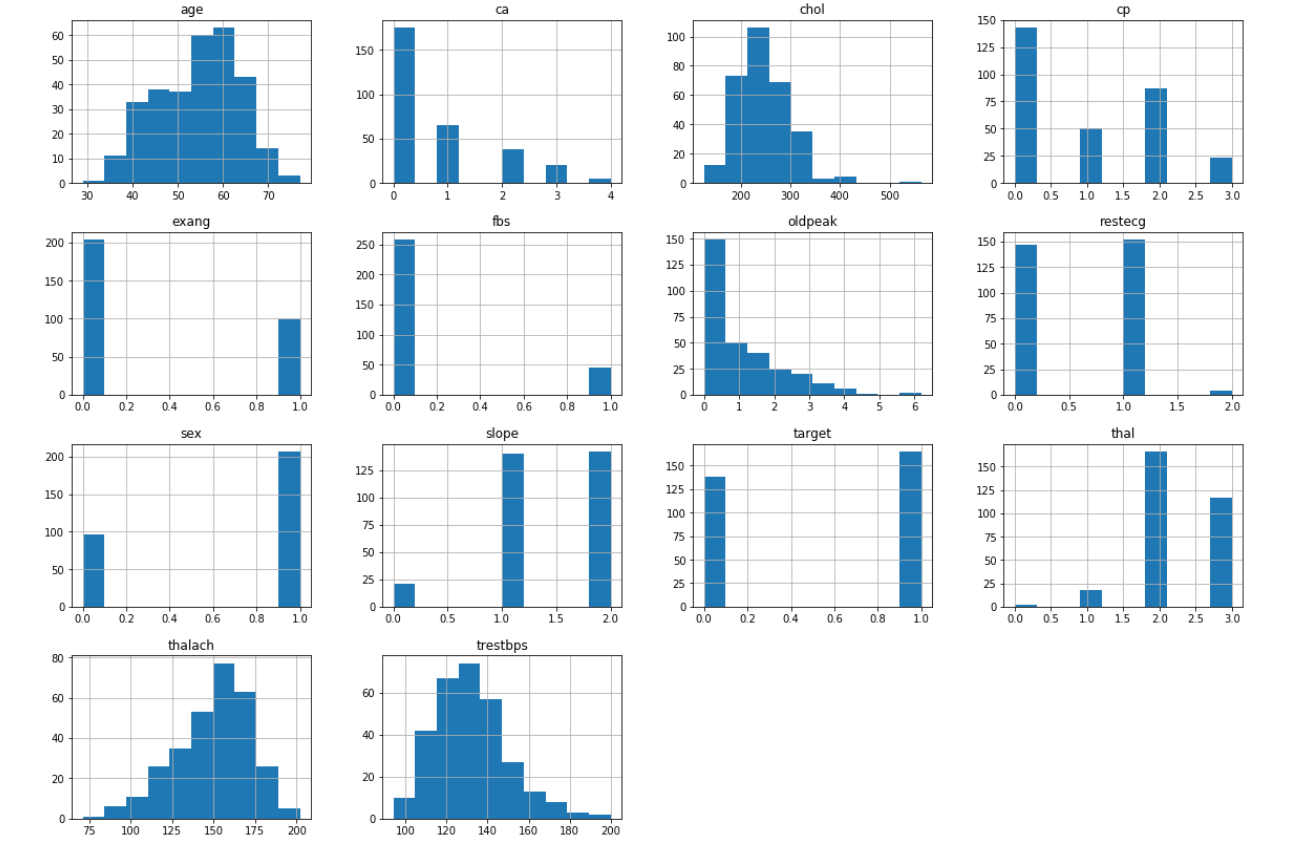
\includegraphics[scale=0.4]{images/hearthistogram.png}
    			\end{center}
	    		\begin{center}
	    			Figure 1.1 Histograms - Cleveland Heart Disease Dataset
	    		\end{center}
    \end{figure}
	
    \pagebreak
    The Count of each target class for the given dataset is as depicted below. The two target classes are:
    \begin{itemize}
    	\item 0: The instances that don’t have heart disease.
    	\item 1: The instances that have heart disease.
    \end{itemize}

	\begin{figure}
		\begin{center}
			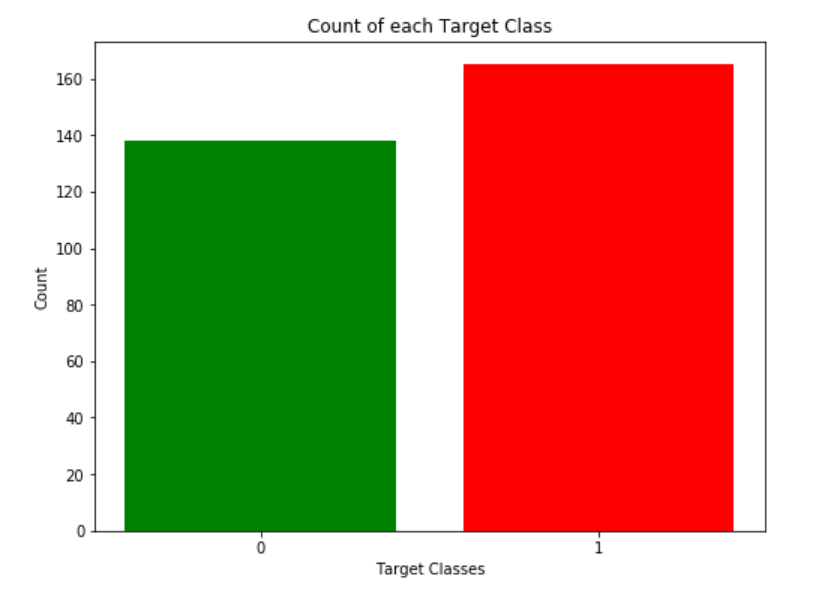
\includegraphics[scale=0.4]{images/heartcount.png}
		\end{center}
		\begin{center}
			Figure 1.2 Frequency Count of the Target Class
		\end{center}
	\end{figure}
	
	\subsubsection{Pima Indians Diabetes Dataset}
	
	This dataset is initially from the National Institute of Diabetes and Digestive and Kidney Diseases. The goal of the dataset is to analytically foresee whether a patient has diabetes, in view of certain diagnostic estimations included in the dataset. The dataset comprises of $768$ individual clinical reports in which $500$ don't have any sickness. In this dataset all the patients are females of atleast $21$ years old of Pima Indian Heritage. 
	The dataset consists of $8$ features shown below:
	\begin{itemize}
		\item Pregnancies
		\item Glucose
		\item Blood Pressure 
		\item Skin Thickness
		\item Insuline
		\item BMI
		\item Diabetes Pedigree Function
		\item Age
	\end{itemize}
	The involvement of each attribute with respect to the number of instances are shown in Figure 1.3:
	\linebreak
	\begin{figure}	
		\begin{center}
			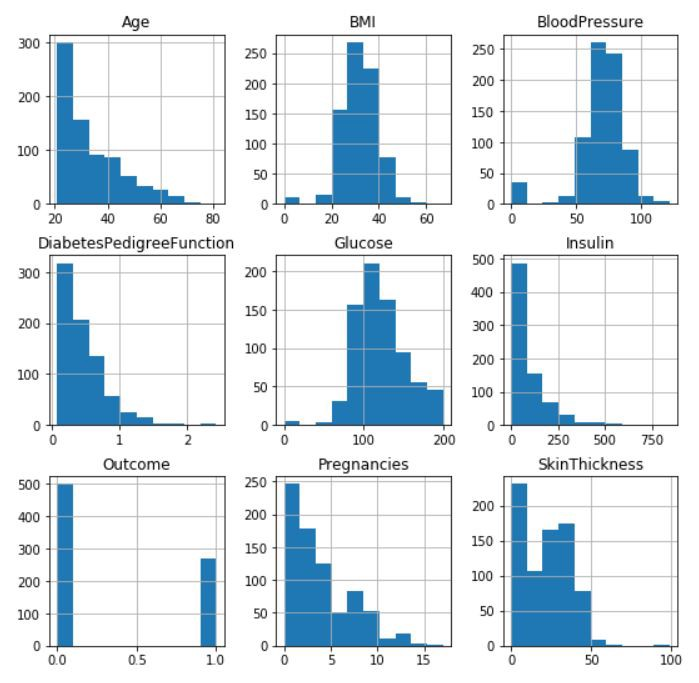
\includegraphics[scale=0.6]{images/diabeteshistogram.jpeg}
		\end{center}
	
		\begin{center}
			Figure 1.3 Histograms - Pima Indian Diabetes Dataset
		\end{center}
	\end{figure}
	\pagebreak
	The count of each target class for the given dataset is as depicted in Figure 1.4.
	\\
	The two target classes are:
	\begin{itemize}
		\item 0: The instances that don’t have diabetes.
		\item 1: The instances that have diabetes.
	\end{itemize}

	\begin{figure}	
		\begin{center}
			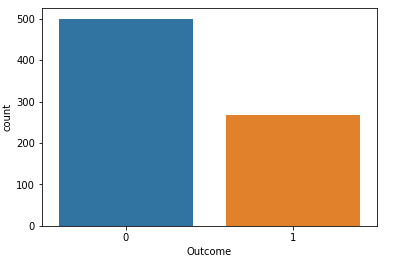
\includegraphics[scale=0.6]{images/diabetescount.png}
		\end{center}
		\begin{center}
			Figure 1.4 Frequency Count of the Target Class
		\end{center}
	\end{figure}
    
 
    
   \section{Summary of Gaps identified}
   Medical diagnosis is considered as a noteworthy yet unpredictable errand that should be done accurately and proficiently. The robotization of the equivalent would be exceptionally helpful. Clinical choices are frequently made dependent on doctor's instinct and experience as opposed to the knowledge of rich information covered up in the database. This training prompts undesirable inclinations, mistakes and extreme medical costs which influences the nature of administration gave to patients. Information mining can create an information-rich condition which can help to essentially improve the nature of clinical choices.
   
   
   
   	\section{Project problem statement and Objective}
   
   	\subsection{Problem Statement}
   	Doctors rely on common knowledge for treatment. When common knowledge is lacking, studies are summarized after some number of cases have been studied. But this process takes time, whereas if machine learning is used, the patterns can be identified earlier
   	For using machine learning, a huge amount of data is required. There is a very limited amount of data available depending on the disease. Also, the number of samples having no diseases is very high compared to the number of samples having the disease.
   	
   	\subsection{Objectives of the project}
   	\begin{enumerate}
   		\item The proposed system predicts heart diseases as well as the chances of diabetes.
   		\item Currently, there is no platform available which helps the users to predict the chances of heart disease and diabetes. We aim to build a powerful platform(web app) which helps the users to predict diabetes and heart disease.
   	\end{enumerate}
   
   
   	\section{Organization of the Report}
  	 The current chapter deals with the detailed Introduction of the project followed by the social and economical impacts of the project. The chapter also contains with the details of all the related research work carried out in this field.
  	 \\
  	 The organization of the remainder of the report is as per the following:
  	 \begin{itemize}
  	 	\item \textbf{Chapter 2}: This section contains the high-level structure of the proposed model alongside the software development methodologies utilized by the project developers during the advancement of this undertaking.
  	 	\item \textbf{Chapter 3}: This chapter contains the design details and UML diagrams of the model along with the data structures and algorithms used in this project.
  	 	\item \textbf{Chapter 4}: This chapter includes the implementation level information of the aforementioned project.
  	 	\item \textbf{Chapter 5}: The testing details of the final model is included in this chapter.
  	 	\item \textbf{Chapter 6}: This part of the report contains the final conclusion drawn along with the future scope of this project.
  	 \end{itemize}
    
     \chapter{High-level Design}
    
   	This chapter covers the software engineering modules on which this project is designed. First, we briefly describe the incremental model, which includes several cycles after which the current version of the web app has been obtained. Then, there is the definition of agility which means regular check of the status of the project by the faculty panel and the project guide. We then briefly describe the Scrum, namely the regular meetings that we had with the team members.
    \section{Software Development Methodology}
    	Software Development Life Cycle (SDLC) is a technique for setting up, creating and testing available programming from merchants (as in Figure 2.1). Sending better programming from the SDLC means that the client meets or exceeds the client's expectations. SDL is a technology used for a product's project, a product's association. This includes creating, maintaining, abusing, and improving programming features. The figure below is a graphic example of the various stages of a typical SDLC.
    	
    	\begin{figure}
    		\begin{center}
    			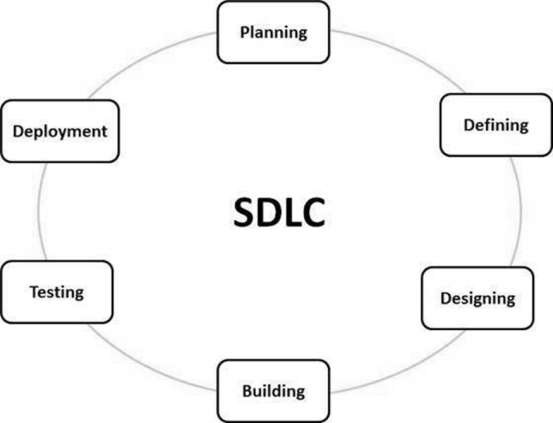
\includegraphics[scale=0.8]{images/sdlc.png}
    		\end{center}
    		
    		
    		\begin{center}
    			Figure 2.1 Software Development Life Cycle
    		\end{center}
    	\end{figure}
    
    	\paragraph{}
    	The detailed SDLC outline (Figure 2.1) shows how all the steps have been contributed to make the proposed work accurate and precise.
    	A typical software development lifecycle consists of the following steps:
    	
    	 \subsection{Stage 1: Planning and Requirement Analysis}
    	The simulation test is the most important and central stage in the SDLC. This is done by the elderly people in the group with significant participation from clients, business offices, advertising studies, space specialists in the business. This data was later used to adjust the required operational procedures and to keep the devil's ability to understand effective, operational and specific zones. The process of standardized certification requirements is tailored to the curriculum and evidence of risk-related risks similar to that in the Master Mining stage. The result considers the outcome of a very specific decision to describe important specific ways of insight, which can be done after a minute's careful understanding of the task.
    	
    	\subsection{Stage 2: Defining Requirements}
    	Once the required test is completed the stage will then be able to image and report the needs of the product and get help from customers or marketing agents. This is done through an SSR (Software Requirements Explanation) report, which contains the essentials to be had and is created during the life cycle.
    	
    	\subsection{Stage 3: Designing the Product Architecture}
    	A systematic approach clearly defines all the plan modules of the item accordingly with the appearance of the data flow and the external and non-modular models (to expect one). Within the framework of the significant number of proposed design models, the unconditional components in the DDS must be minimized.
    	
    	\subsection{Stage 4: Building or Developing the Product}
    	Real change begins in this period of SDLC, and things are made. DDS generates programming code during this stage. If the arrangement is performed in a positive and positive way, the code can be a long life problem. The developers should go after their representation of these code rules and use their affiliation and programming gadgets such as code compilers, middlemen, checker debuggers, etc. to generate the code. Separate state-of-the-art programming programmers for coding, for example C, C ++, Pascal, Java, and Python are used. The programming language is used to select the type of computer programs to write.
    	
    	\subsection{Stage 5: Testing the Product}
    	This stage is usually a part of a wider number of stages, as in the front-line SDLC model, testing processes are generally two-connected with each period of the SDLC. However, this phase checks that the bus, after representing something, has grown, settled and re-examined, until it meets the quality measures shown in the SRS.

    	\subsection{Stage 6: Deployment in the Market and Maintenance}
    	 Once this item is tried and arranged to pass it is regularly issued in the right market. The remodeling now and again begins in phases, as evidenced by this affiliate business strategy. The first thing may be issued in a limited area and tried in a valid business state (UAT-User affirmation testing) then in view of the information, the item can be released as it is or parcel of promotion. With the proposed changes to focus on. After releasing the item into the market, its upbringing has improved the condition of existing customers.
    	
    	\section{Architecture}
    	
    	\begin{figure}
    		\begin{center}
    			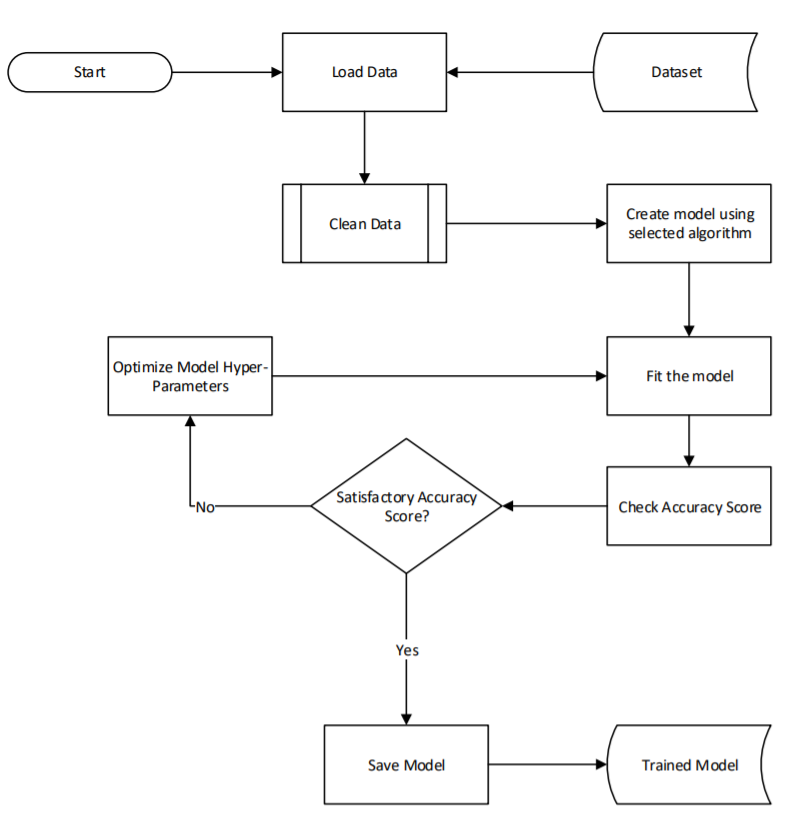
\includegraphics[]{images/df.png}
    		\end{center}
    		
    		\begin{center}
				Figure 2.2: Initial design of the proposed system
    		\end{center}
    	\end{figure}
    	
    	
    	This report will provide a result that is distributed into three phases:
    
    	\begin{enumerate}
    		\item \textbf{Analysis Phase (Based on the Dataset): } At this stage, the main concentration is to examine the information from the data set and to illuminate the patient's medical data. At this stage, we try to analyze which medical data or medical values have the greatest impact on disease prognosis and which features have the least impact.
    	\item \textbf{Combining analysis stage with the parameters:} At this stage, we give some conditions based on the patient's condition (whether the patient is suffering from heart disease and diabetes). The application applies various machine learning algorithms to generate a module, which in turn is used in the prediction process.  
    	\item \textbf{Prediction Phase:} At this stage, we disclose the results and declare the possibility that the person is suffering from heart disease or diabetes. The results were predicted using different machine learning algorithms from user-defined values.
    	\end{enumerate}
    	
    	\section{Incremental Model}
    	
    	The incremental frames represent a strategy for programming movement where something is designed, processed and maximized (until some degree more solid each time) until the task is completed. 2.2). It both turns and comes back down. Things get caught up when he caters to the more prominent part of his needs. This indicates that the datasets of the waterfall appeared on a civilizational basis of the prototype. The item is delivered in separate sections, each of which is organized and structured in an anonymized way (together with the name). Each part is sent to the client when it is completed. This gift avoids the use of products and maintains a strategic distance from long growth times. It likewise guarantees the removal of an important starting capital and the shortage period. This shows that growth spurt is at the same time promoting the frightening effects of modern systems at the same time.
    	\paragraph{}
    	Characteristics of the Incremental Model:
    	\begin{itemize}
    		\item System is isolated into various small units.
    		\item Partial systems are meant to deliver the ultimate framework.
    		\item Firstly the required procedures are performed.
    		\item What is required is cemented when an extended bit is produced.
    	\end{itemize}
    	
    	
    	\begin{figure}
    		\begin{center}
    			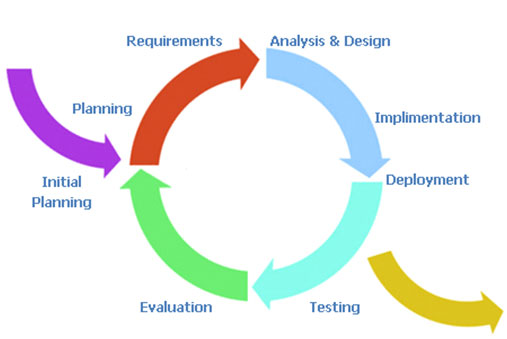
\includegraphics[]{images/cycle.jpg}
    		\end{center}
    		
    		
    		\begin{center}
    			Figure 2.3: Incremental model for project
    		\end{center}
    	\end{figure}
    	After each cycle, backward testing is facilitated. In the midst of this test, the damaging parts of the product can be seen lightly so that some changes can be made internally at any one stress. It is, in general, easy to examine and explain the different approaches to the programming movement in light of the ways in which the eight-part changes are made today between each section. It focuses more on the center and takes the internal scrutiny of each section seriously. The customer seems to respond to highlighting and evaluating the product being used for any desired changes. The essential thing is the faster and lower cost of the accelerator model.
    	
    	\section{Agility and Scrum}
    	Advanced programming can be a strategy for creating programming techniques (such as another programming reverse systems - waterfall model, V-model, incremental shows etc.). In English, detectors mean the ability to move quickly and easily, and reacting quickly is often an important piece of well-structured programming reversals.
    	In traditional expert programming such as Waterfalls model, an outage can take several months and a long time because the client may not get the opportunity to see the end result of that commitment. In the exceptional case, the non-Agile assignments determine the timeframe for submission, arrangement, development, testing and client acceptance testing failures, spray work done sprints or attributes that are in term today (sprint) / Squares can move from 2 weeks to 2 months) in the midst of selected skills.
    	
    	\subsection{Agility and the cost of change}
    	The standard method of considering in programming movement (upheld by various quite a while of experience) is that the got of advance increments nonlinearly as an endeavour advances (Figure 2.3). It is fairly fundamental to oblige an adjust when a thing pack is gathering essentials (exactly on schedule in a meander). A use situation must be changed, a summary of limits likely could be widened, or a made explicit can be changed. The expenses of accomplishing this work are irrelevant, and the time required won't inauspiciously sway the consequence of the endeavour. Be that as it may, imagine a circumstance where we quick forward various months. The bundle is in the midst of endorsement testing (something that occurs generally late inside the meander), and a fundamental associate is asking for an indispensable suitable change. The adjust requires a change to the compositional orchestrate of the thing, the graph and progression of three present-day parts, modifications to another five sections, the arrangement of unused tests, etc.
    	
    	
    	\begin{figure}
    		\begin{center}
    			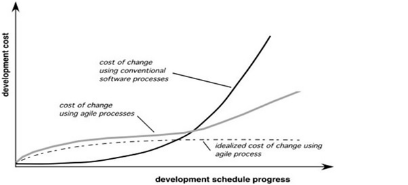
\includegraphics[scale=0.7]{images/chotu.png}
    		\end{center}
    		
    		
    		\begin{center}
    				Figure 2.4: Agility and the cost of change
    		\end{center}
    	\end{figure}

    	\paragraph{}
    	\textbf{Advantages of Agile Methodology:}
    	\begin{itemize}
    		\item In Dexterous framework the advancement of making PC programs is unremitting. 
    		\item The customers are satisfied considering the truth that after each Sprint, the working segment of the thing is given to them. 
    		\item Clients can see the working part which fulfilled their needs. 
    		\item in the event that the customers have any analysis or any change inside the bit by then it tends to be obliged inside the show area of the thing. 
    		\item In Spry framework, the bit by bit affiliations are required between the bosses and the creators. 
    		\item In this framework thought is paid to the great diagram of the thing.
    	\end{itemize}
    	
    	
    	
    	\section{Scrum}
    	Scrum could be a quick structure for organizing work with a feature on programming development. It is organized parties of three to nine fashioners who break their work into works out that should be possible inside time-boxed cycles, called runs (routinely fourteen days) and track advance and re-diagram in 15-minute stand-up social endeavours, called bit by bit scrums. Approaches to deal with sorting out made by differing scrum bundles in increasingly imperative affiliations cement Large-Scale Scrum, Scaled Dexterous System (SAF) and Scrum of Scrums, among others.
    	\subsection{Activities performed by the team in the scrum}
    	\begin{itemize}
    		\item At the initial stages, extension and plan of the project are chosen. 
    		\item Regular commitment on a week by week premise to keep a mind all the exercises are in a state of harmony with one another. 		
    		\item Engagement with the project guide assisted with doing the necessary adjustment of the project.    		
    		\item Requirement gathering was done in a gradual manner.     		
    		\item project was separated into various components with the goal that legitimate appropriation of work should be possible in the group. 
    		\item Each colleague is answerable for its doled out work.    		
    		\item Every 14 days progress was checked and new objectives of the project were characterized to concentrate on.    		
    		\item After the development of each module testing was done to ensure the best possible working of the module.    		
    		\item All the components were coordinated to ensure everything functions admirably together.    		
    		\item Report composing was done on a nonstop premise to catch all the outcomes and conversations.
    	\end{itemize}
    	
    	
    	\begin{figure}
    		\begin{center}
    			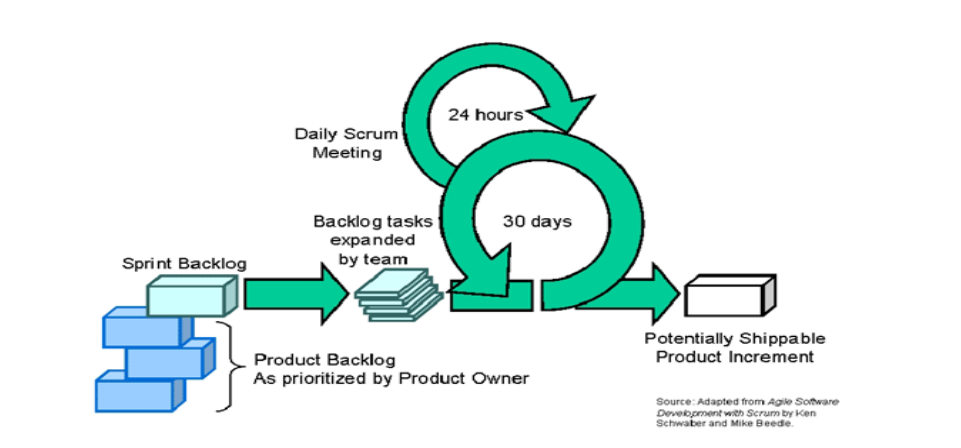
\includegraphics[scale=0.5]{images/animesh_chotu.png}
    		\end{center}
    		
    		\begin{center}
    			Figure 2.5: Scrum design of the project
    		\end{center}
    	\end{figure}
		\paragraph{}
    	Scrum has three roles: Product Owner, Scrum Master, and Team:
    	\begin{itemize}
    		\item \textbf{Item Owner:} The Item Owner should be careful with trade with vision, pro, and receptiveness. The Item Proprietor is liable for diligently giving the vision and necessities to the change gathering. It's once in a while hard for Product Proprietors to strike the best possible change of thought. Since Scrum regards self-relationship among social events, an Item Proprietor must fight the need. to humbler scale direct. In the meantime, Item Proprietors must be open to answer ask from the social event.
    		
    		\item \textbf{Scrum Master:} The Scrum Master goes around as a helper for the Item Proprietor and the social gathering. The Scrum Ace doesn't deal with the social event. The Scrum Ace attempts to rinse any obstructions that are blocking the social issue from satisfying its run goals. This secures in the social event to stay innovative and valuable while ensuring its triumphs are obvious to the Item Proprietor. The Scrum Ace other than attempts to ask the Item Proprietor around how to create ROI for the social event.
    		
    		\item \textbf{Team:} As appeared by Scrum's facilitator, "the gathering is totally self-dealing with." The advancement all out is fit for self-organizing to add up to work. A Scrum development store up contains around seven totally committed people (officially 3-9), ideally in one social occasion room guaranteed from outside redirections. For programming wanders, a customary get-together hardens a mix of programming engineers, modellers, programming engineers, inspectors, QA specialists, analysers, and UI coordinators.
    	\end{itemize}
    	
    	
    	\section{Functional Requirements}
    	\begin{itemize}
    		\item Predict the probability of Heart Disease and Diabetes with given user inputs.
    		\item Contribute to the dataset or request to add functionalities.
    	\end{itemize}
    
    	
    	\section{Non-Functional Requirement}
    	\paragraph{}
    	Non-rational necessities are prerequisites that exhibit rules that can be utilized to pass judgment on the activity of a structure, as opposed to explicit practices. This could be showed up particularly in association with important prerequisites that portray explicit direct or cutoff points. 
    	\paragraph{} 
    	Non-practical necessities are a noteworthy piece of the time called characteristics of a structure. Unmistakable verbalizations for utilitarian necessities are restrictions, quality attributes, quality targets, nature of association prerequisites and nonbehavioral fundamentals.
    	
    	\section{Feasibility Analysis}
    	\subsection{Technical feasibility} 
    	The project is technically feasible as it very well may be manufactured utilizing the currently accessible advances. It is an electronic application that utilizes the Grails Framework. The innovation required by Disease Predictor is accessible and consequently, it is technically feasible.
    	
    	\subsection{Economic feasibility} 
    	The project is economically feasible as the cost of the project is included uniquely in the deployment of the web-app. As the information tests expands, which devour additional time and handling power. All things considered, a superior processor may be required.
    	
    	\chapter{Detailed Design}
    	This section will cover the design of our model in detail. Firstly with interface design that will provide a detailed explanation about the interface design, and then with the Data Structure and Algorithms that have been used in the project. The whole detailed system design with use case has been shown in Fig 3.1.
    	
    	\section{Interface Design}
    	This section describes about the user’s interaction with the interface. The inter-face designs/screen-shots have been added in order to give a better view of the user Interface.
    	
    	
    		\begin{center}
    			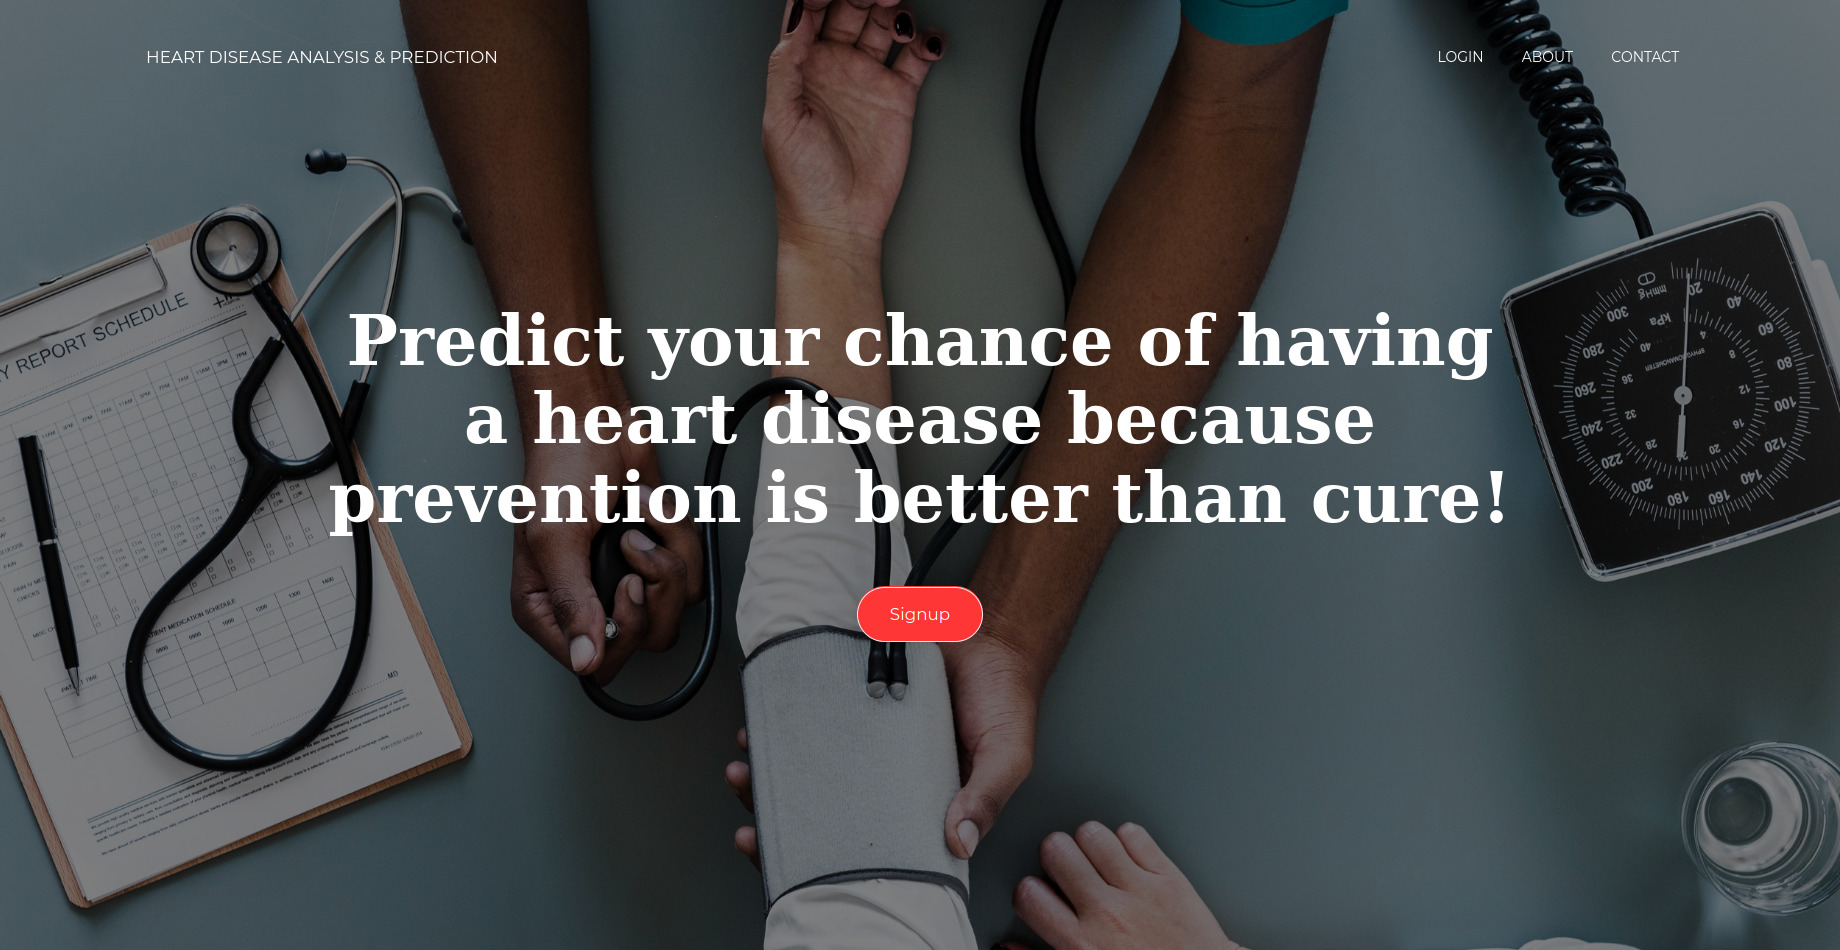
\includegraphics[width=17cm]{Screenshots/home1.jpg}
    			\begin{figure}
    				\caption{Home page }
    			\end{figure}
    		\end{center}
    		
    		\begin{figure}
    				\begin{center}
    				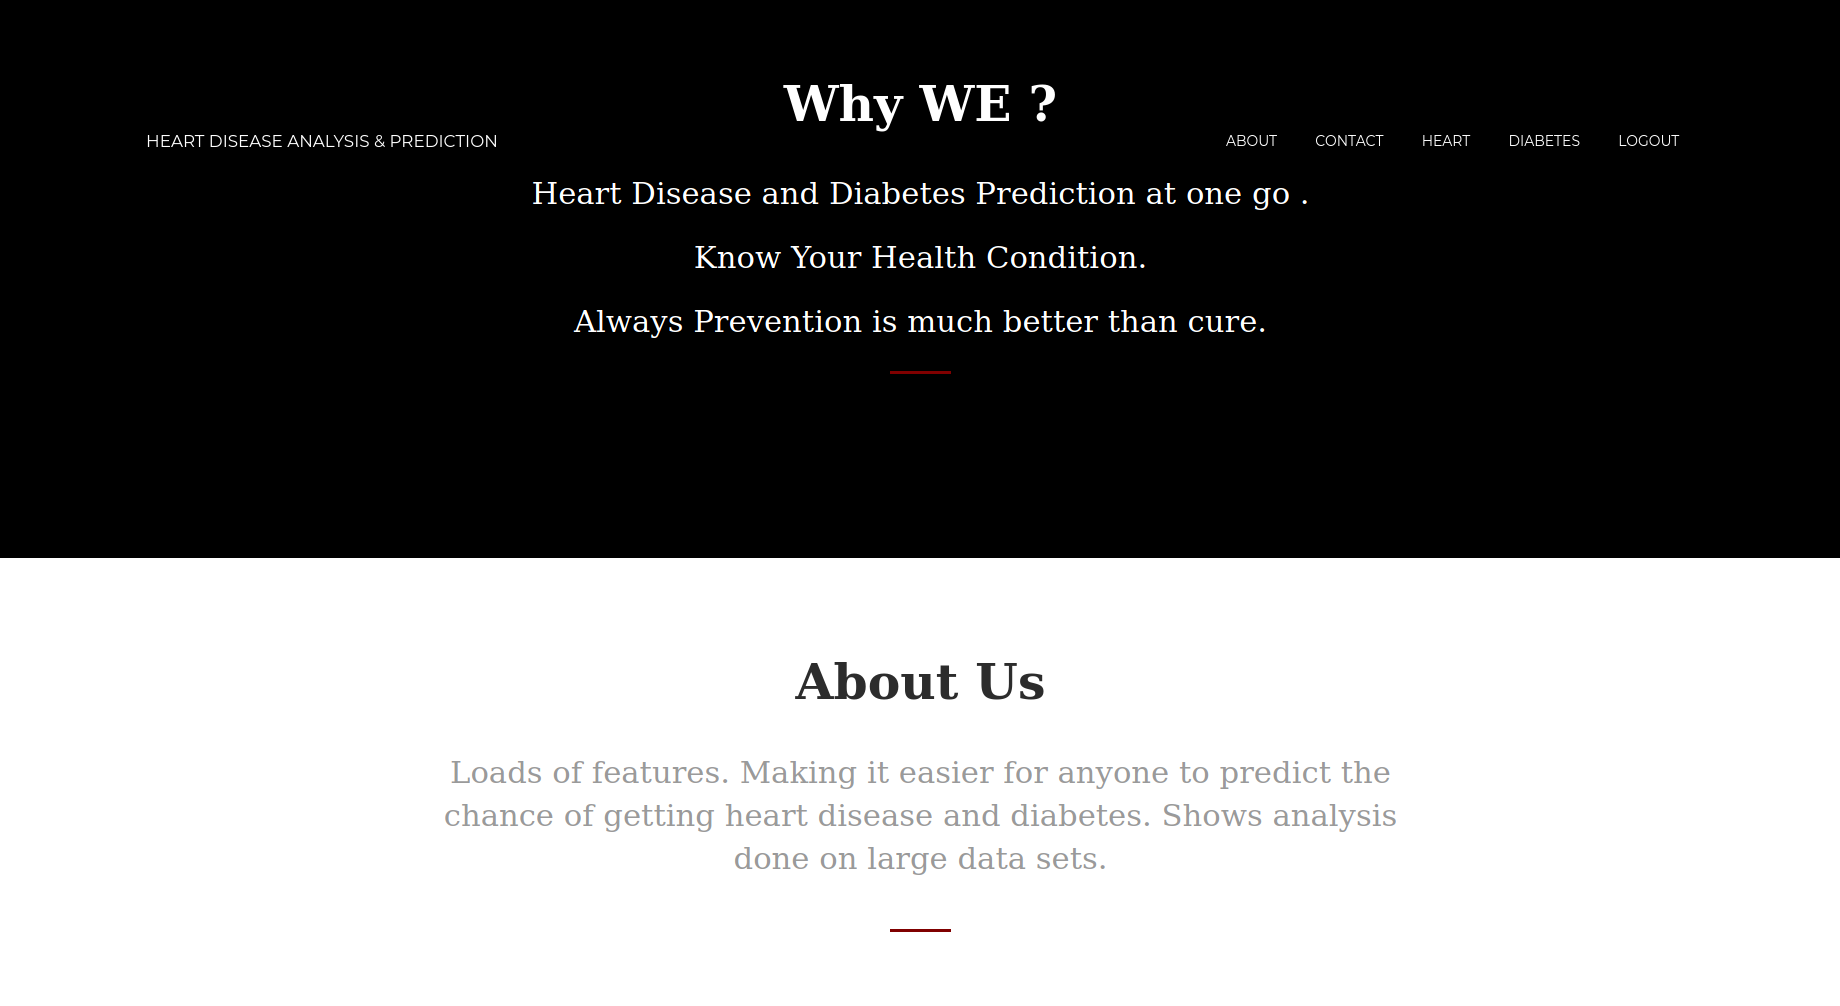
\includegraphics[width=17cm]{Screenshots/home2.PNG}
    				\caption{Home}
    				\end{center}
    		\end{figure}
    		
    		\begin{figure}
    				\begin{center}
    				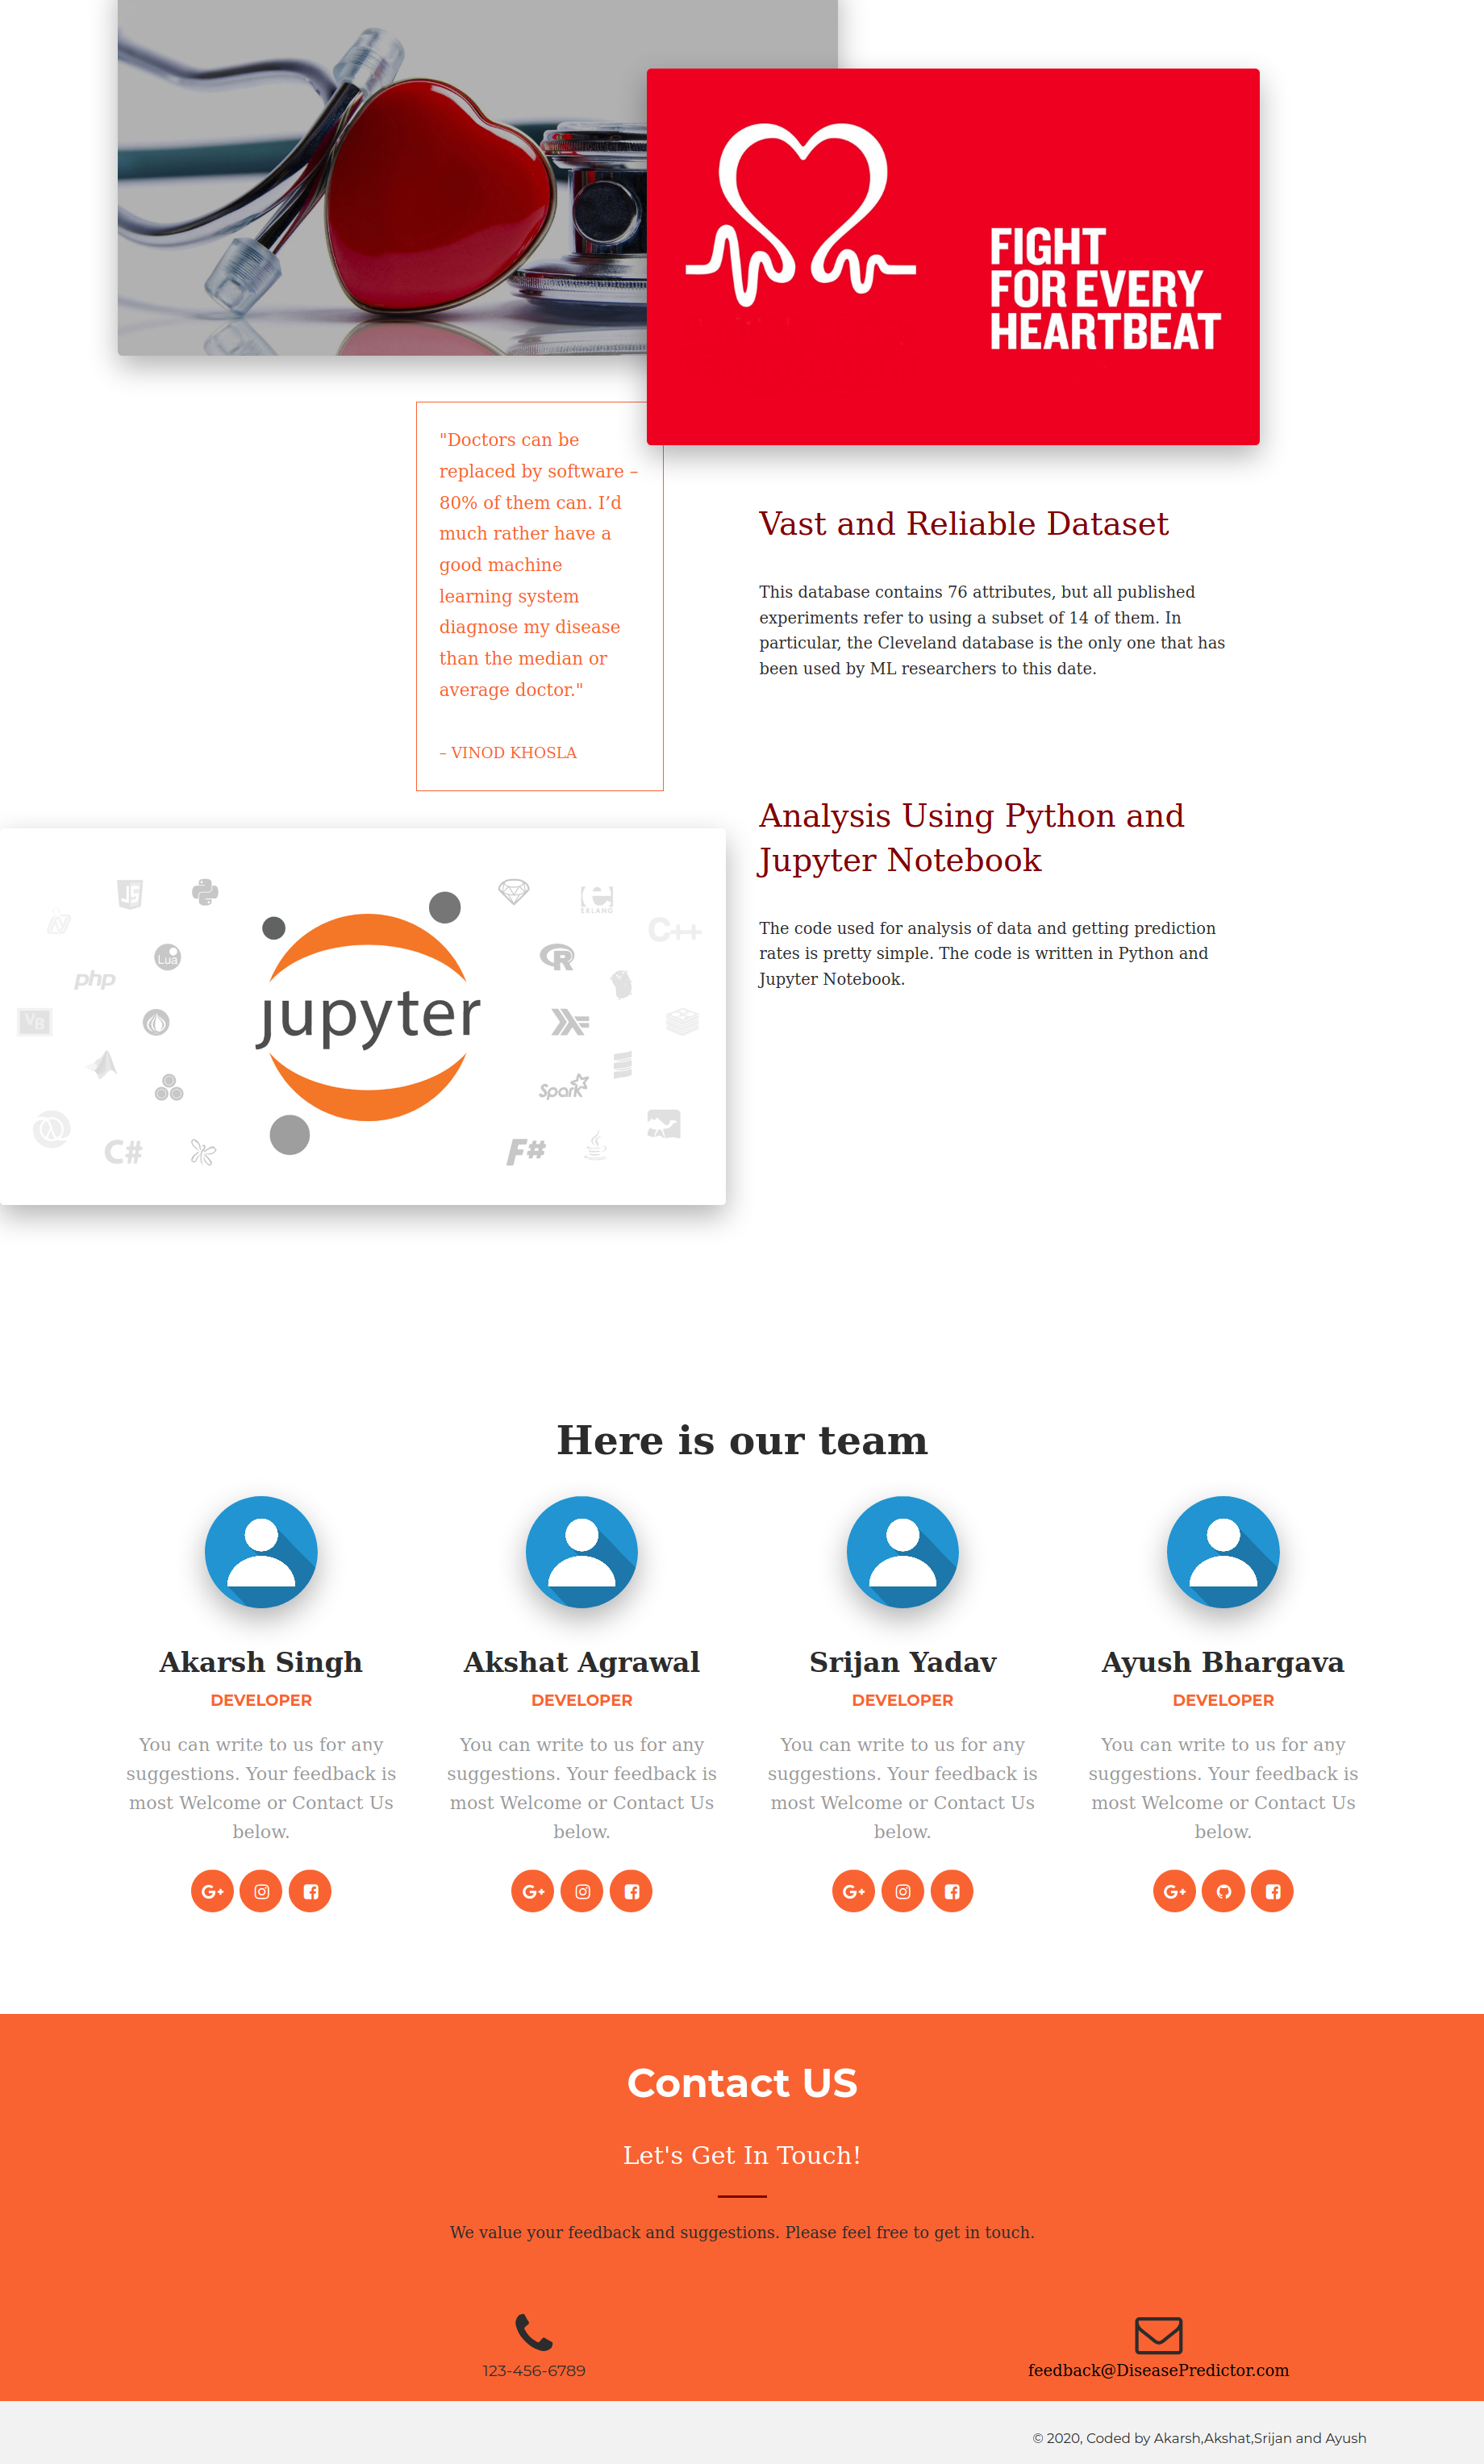
\includegraphics[width=10cm,scale=0.5]{Screenshots/home3.PNG}
    				\caption{Home}
    				\end{center}
    		\end{figure}
    
    			\begin{figure}
    				\begin{center}
    				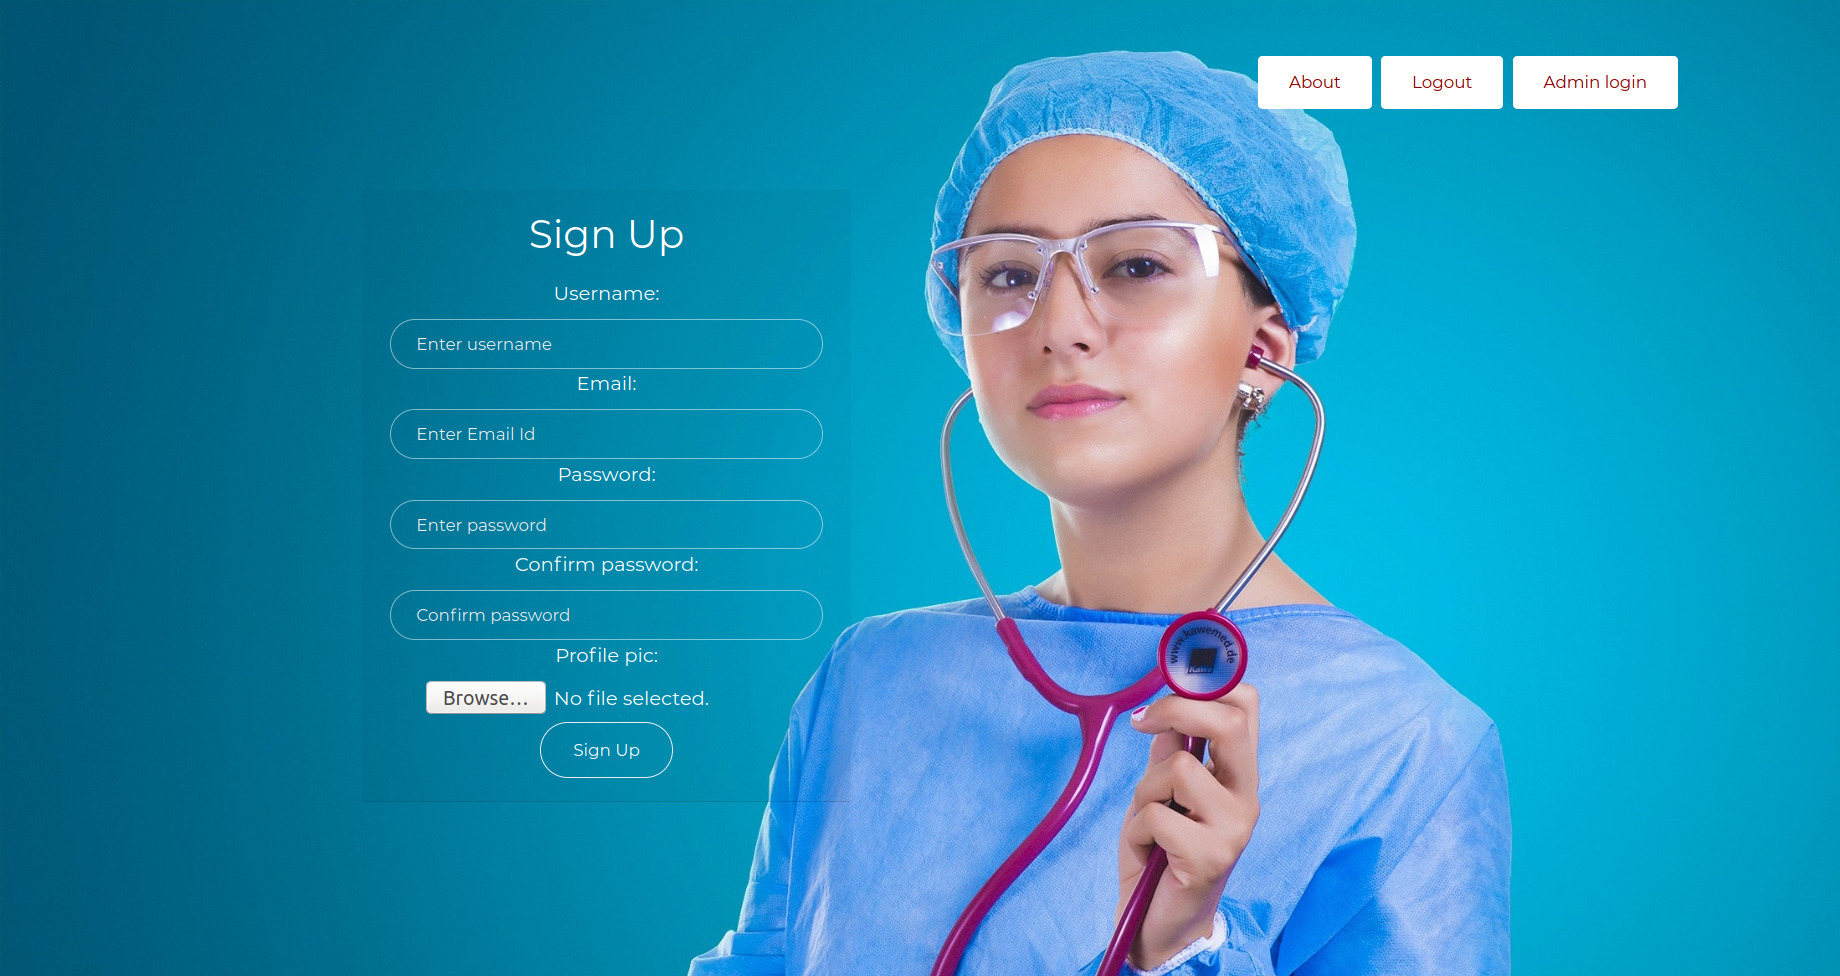
\includegraphics[width=17cm]{Screenshots/sign-up.jpg}
    				
\includegraphics[width=17cm]{Screenshots/login.PNG}
    				\caption{SignUp and Login feature}
    				\end{center}
    			\end{figure}
    			
    			\begin{figure}
    				\begin{center}
    				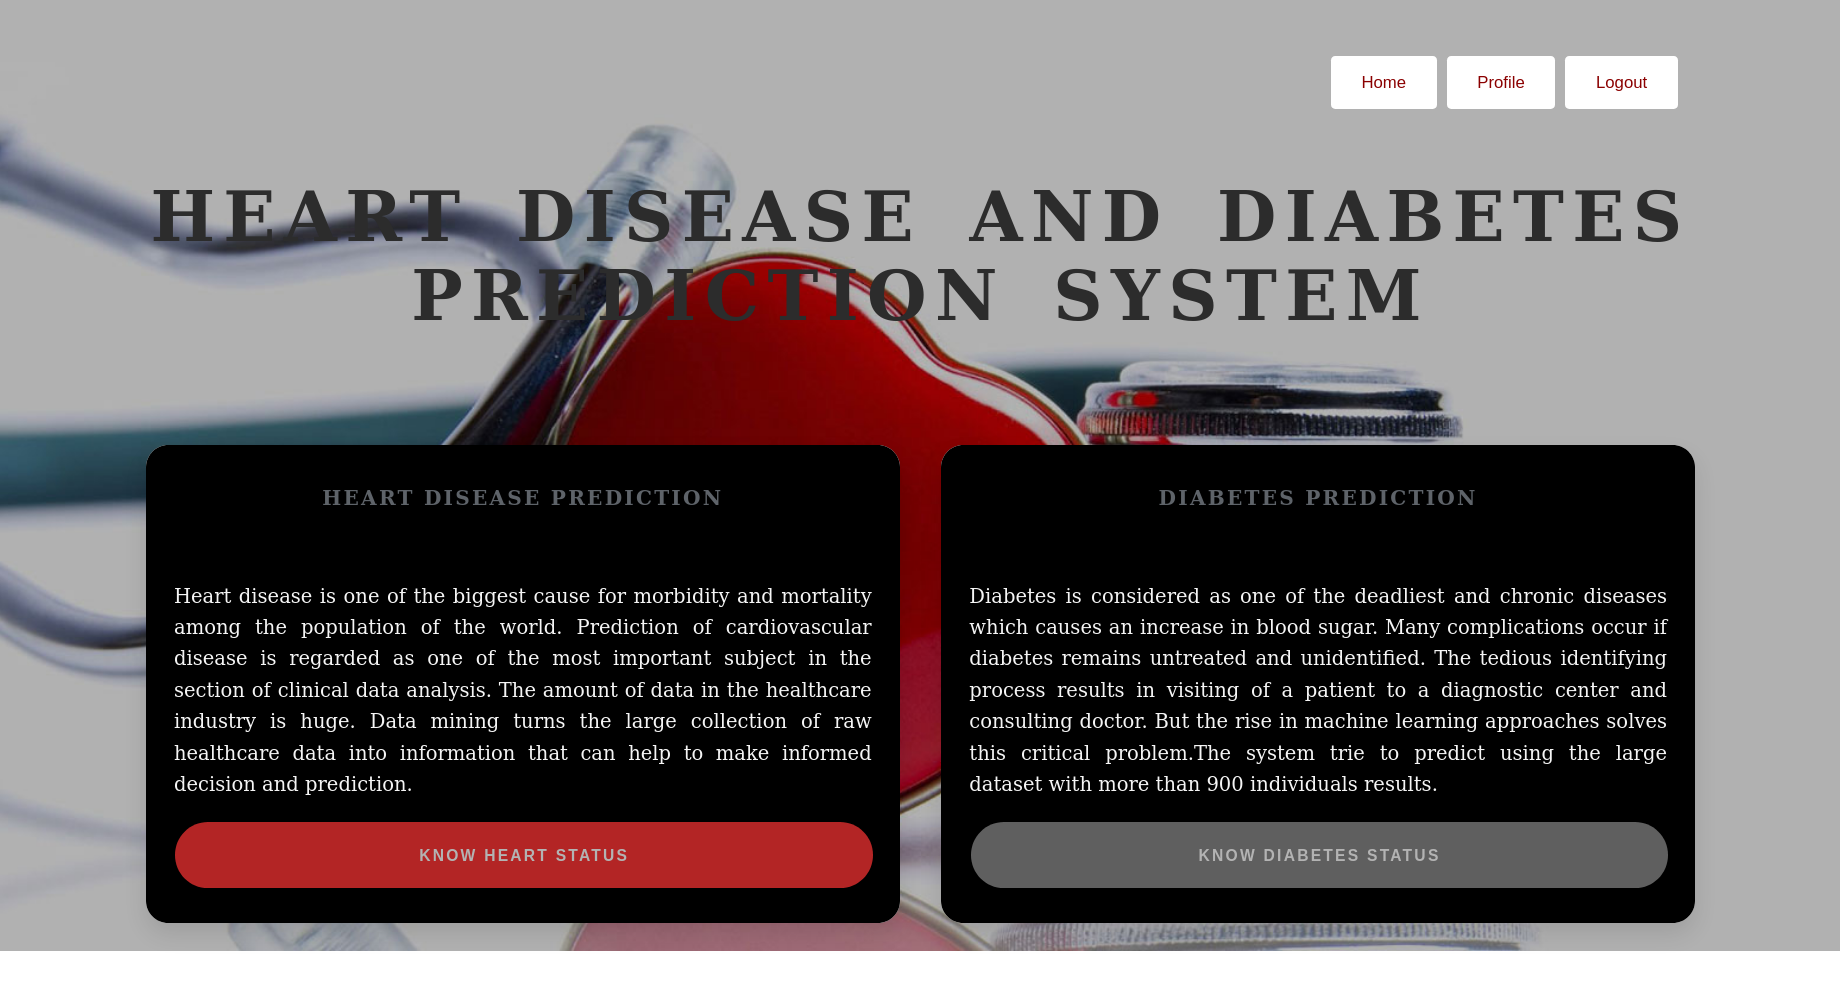
\includegraphics[width=17cm]{Screenshots/description-predict.PNG}
    				\caption{options of Prediction Engine}
    				\end{center}
    			\end{figure}
    			
    			\begin{figure}
    				\begin{center}
    				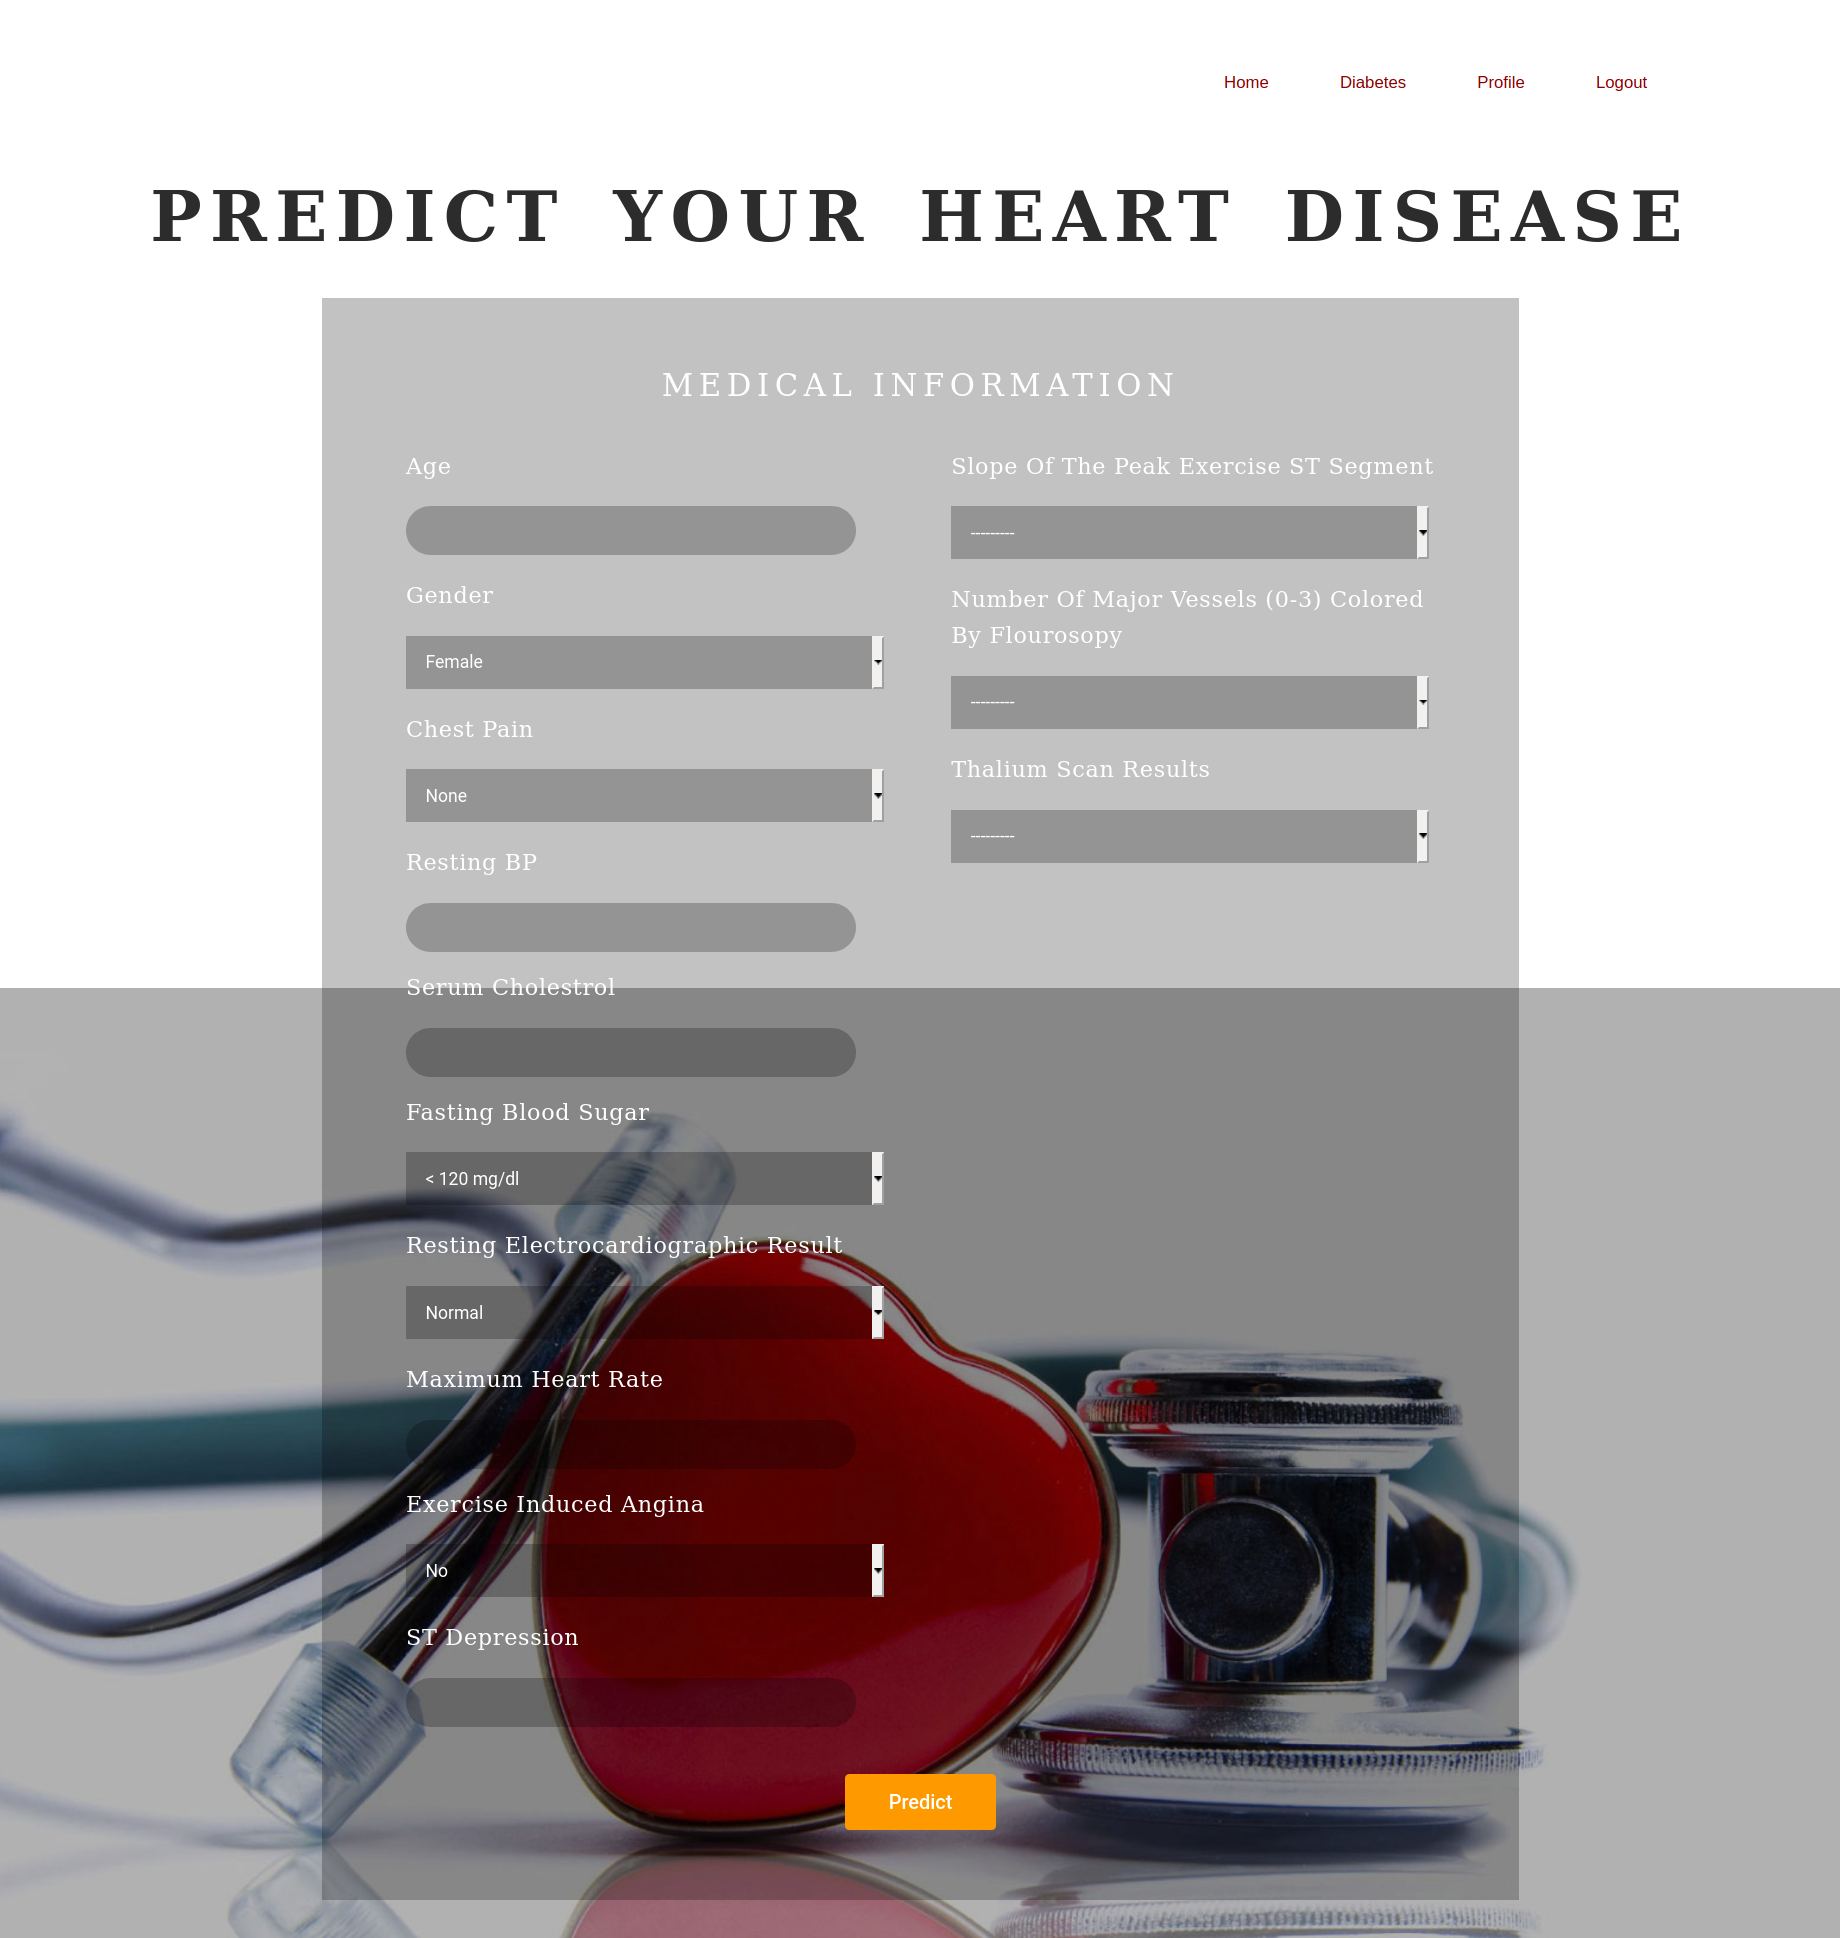
\includegraphics[width=17cm]{Screenshots/heart-form.PNG}
    				\caption{Heart diseases prediction form for patient}
    				\end{center}
    			\end{figure}
    			
    			\begin{figure}
    				\begin{center}
    				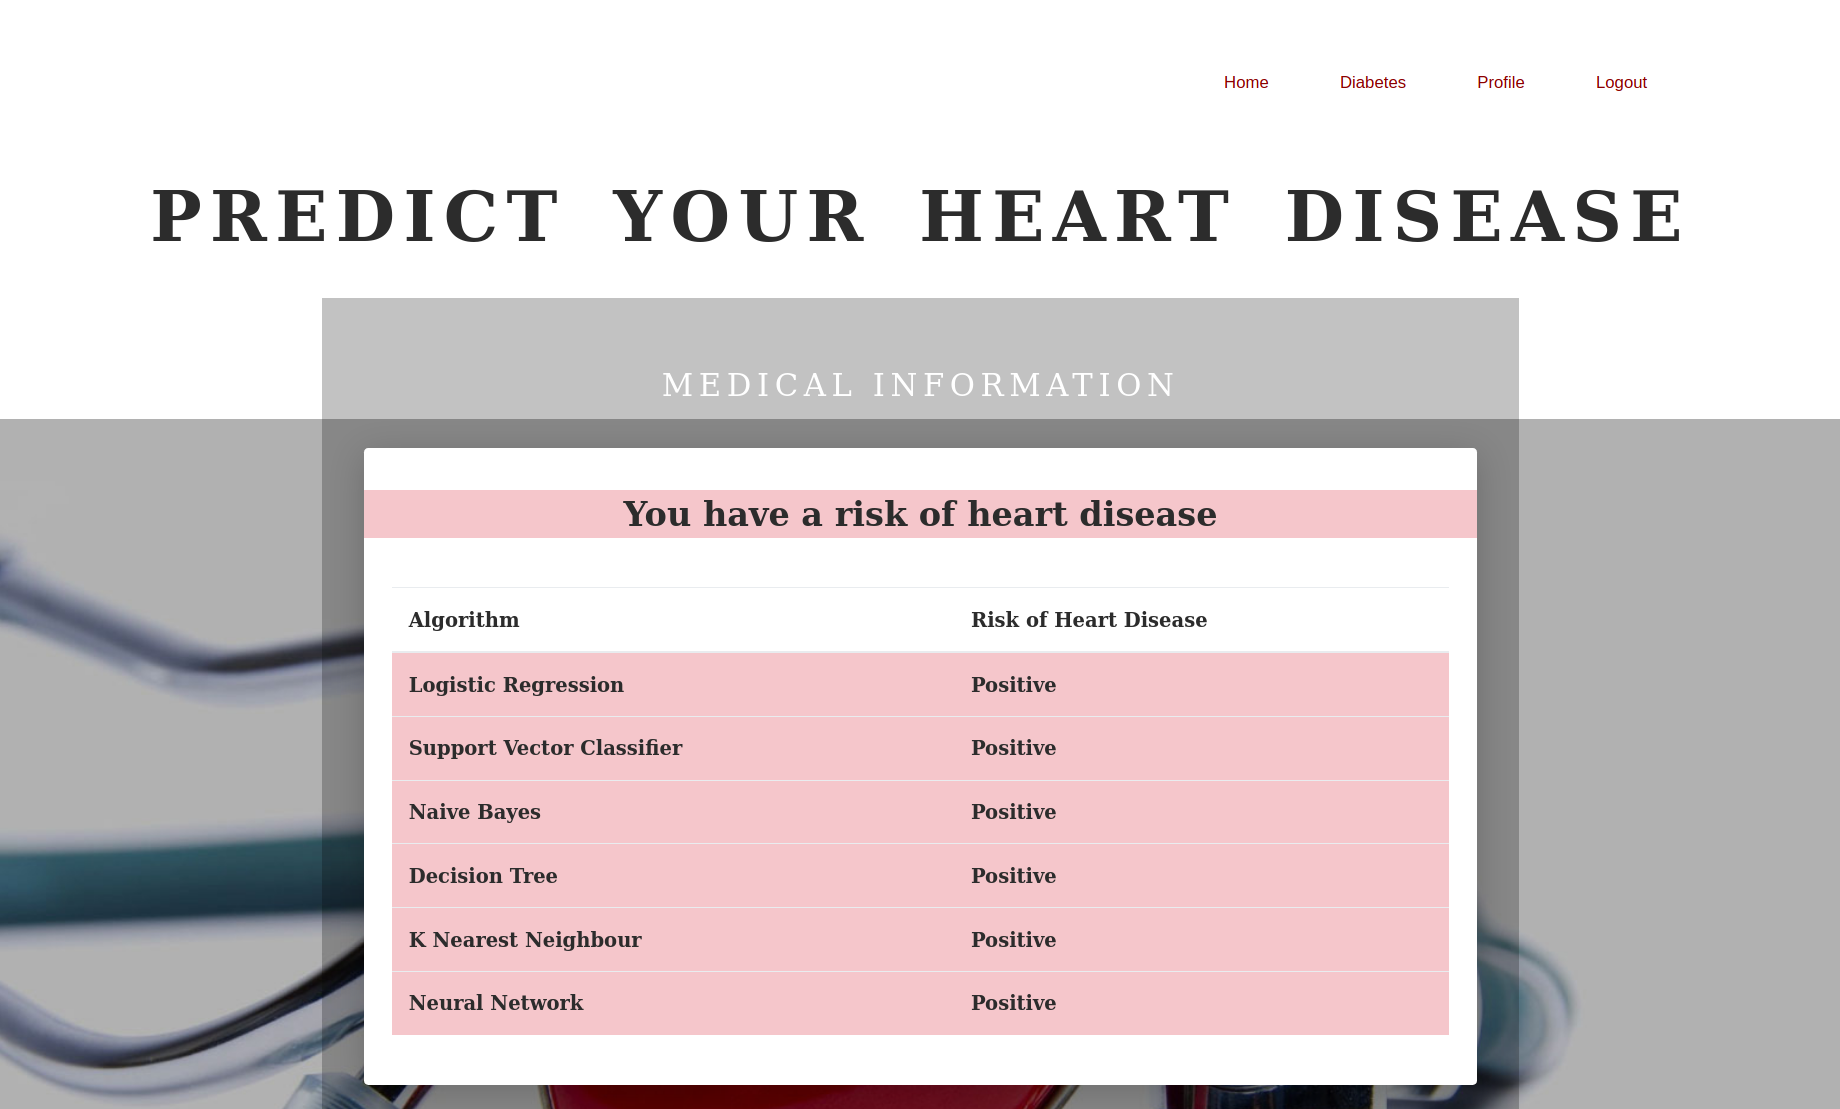
\includegraphics[width=17cm]{Screenshots/heart-result.PNG}
    				\caption{Heart diseases prediction result for patient}
    				\end{center}
    			\end{figure}
    			
    			\begin{figure}
    				\begin{center}
    				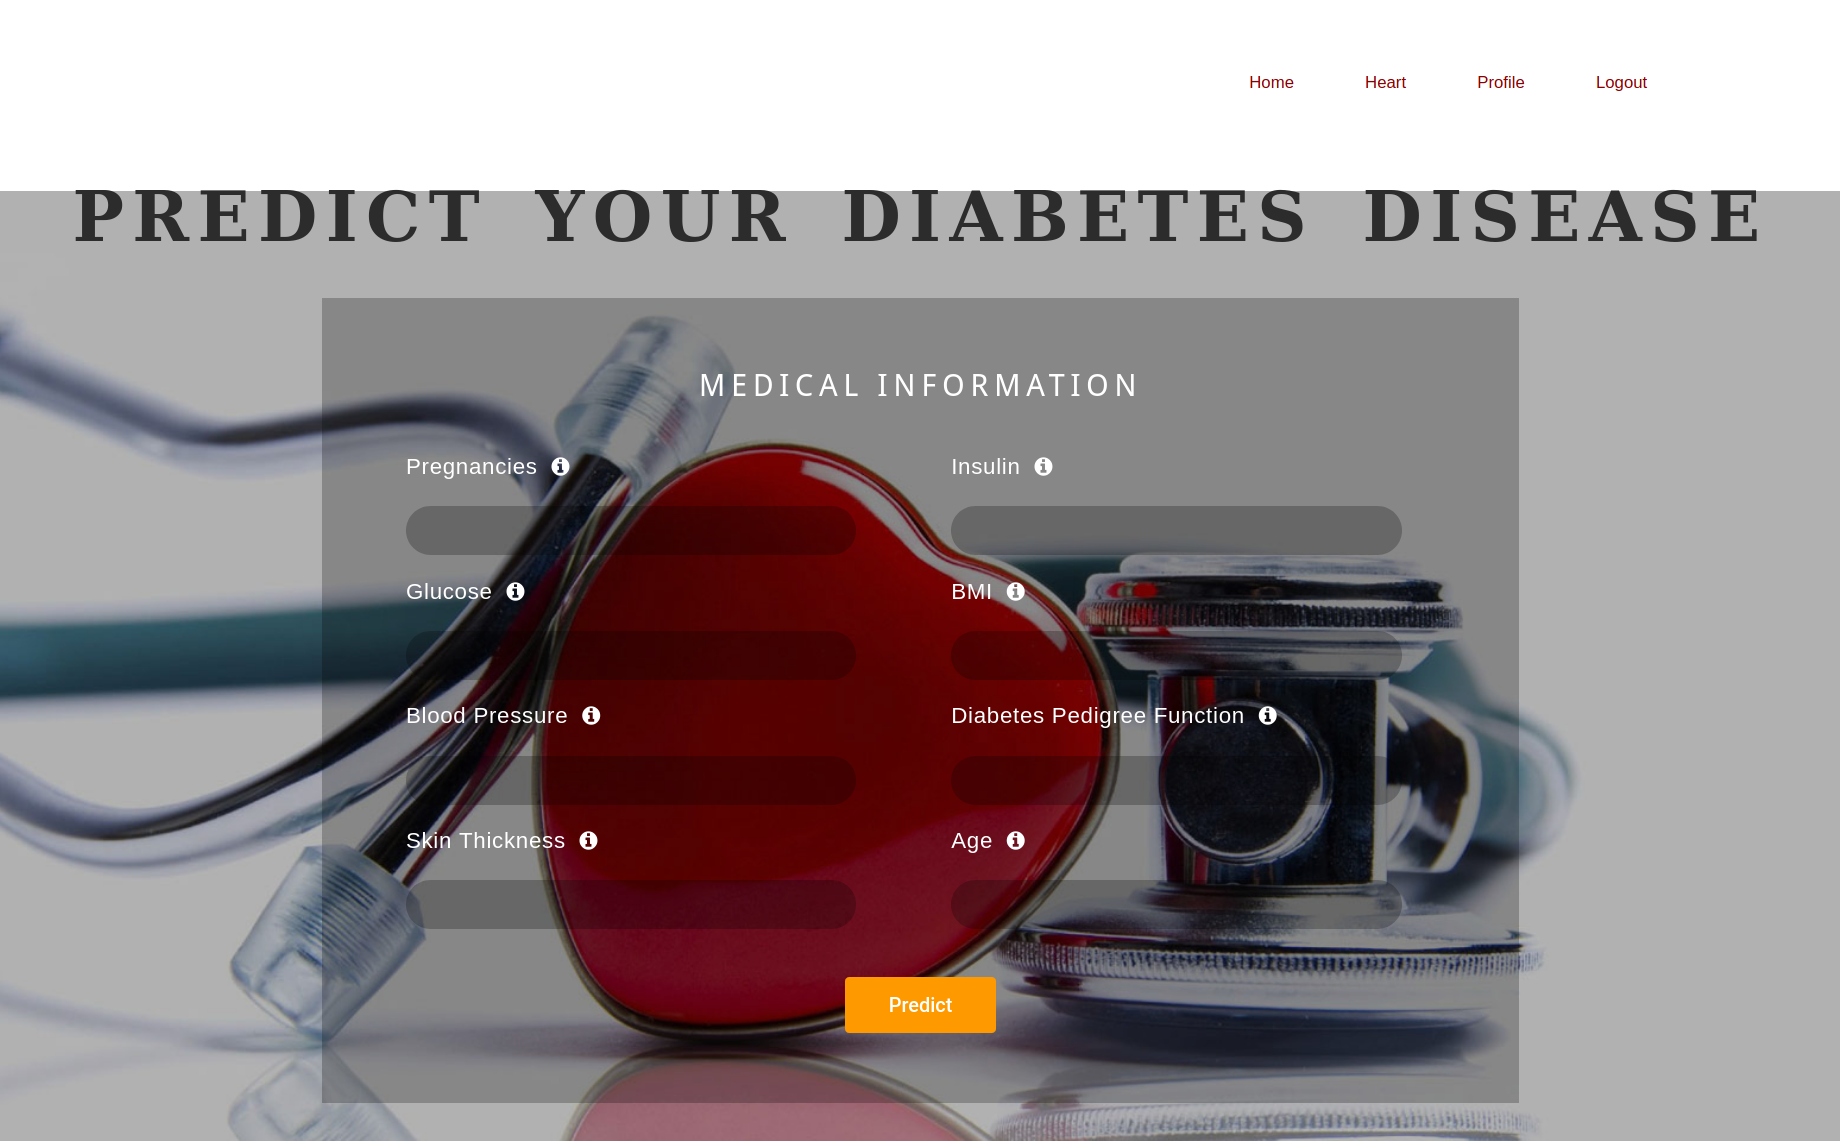
\includegraphics[width=17cm]{Screenshots/diabetes-form.PNG}
    				\caption{Diabetes prediction form for patient}
    				\end{center}
    			\end{figure}
    			
    			\begin{figure}
    				\begin{center}
    				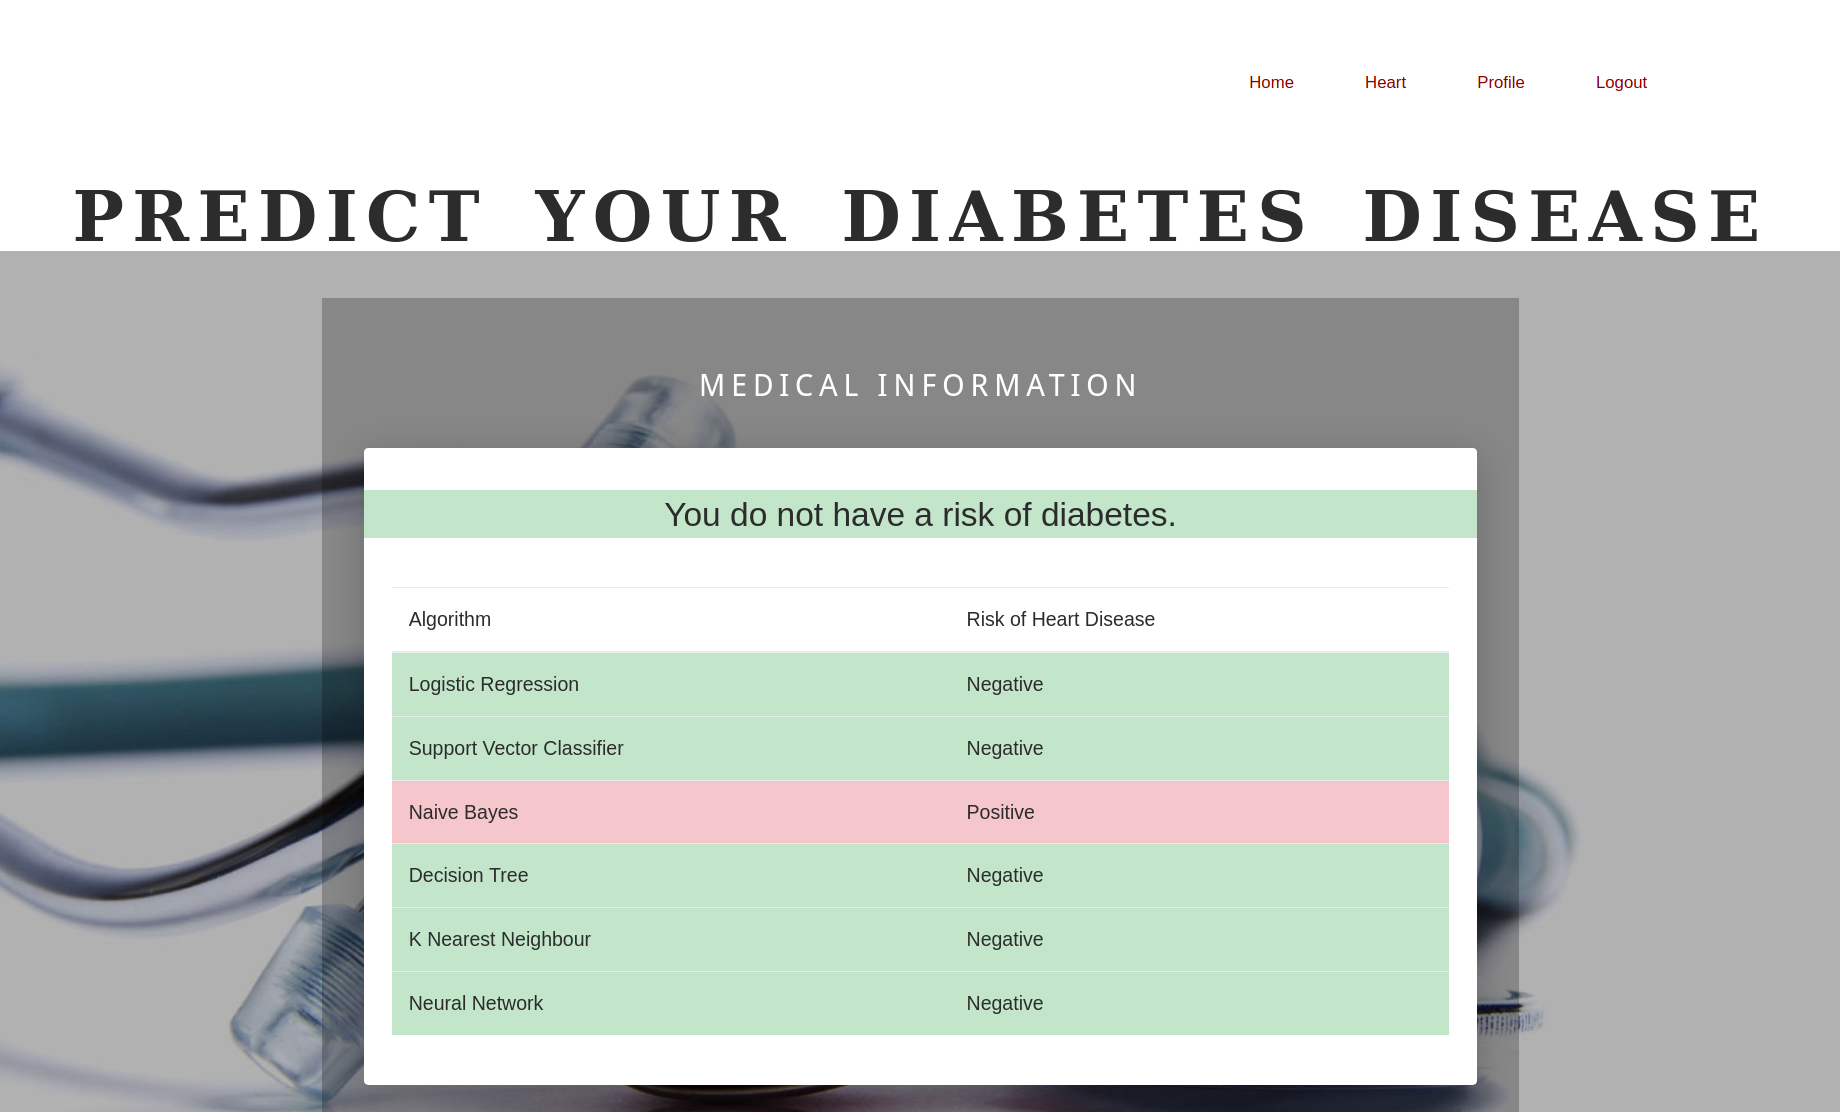
\includegraphics[width=17cm]{Screenshots/diabetes-result.PNG}
    				\caption{Diabetes prediction result for patient}
    				\end{center}
    			\end{figure}
    			
    			\begin{figure}
    				\begin{center}
    				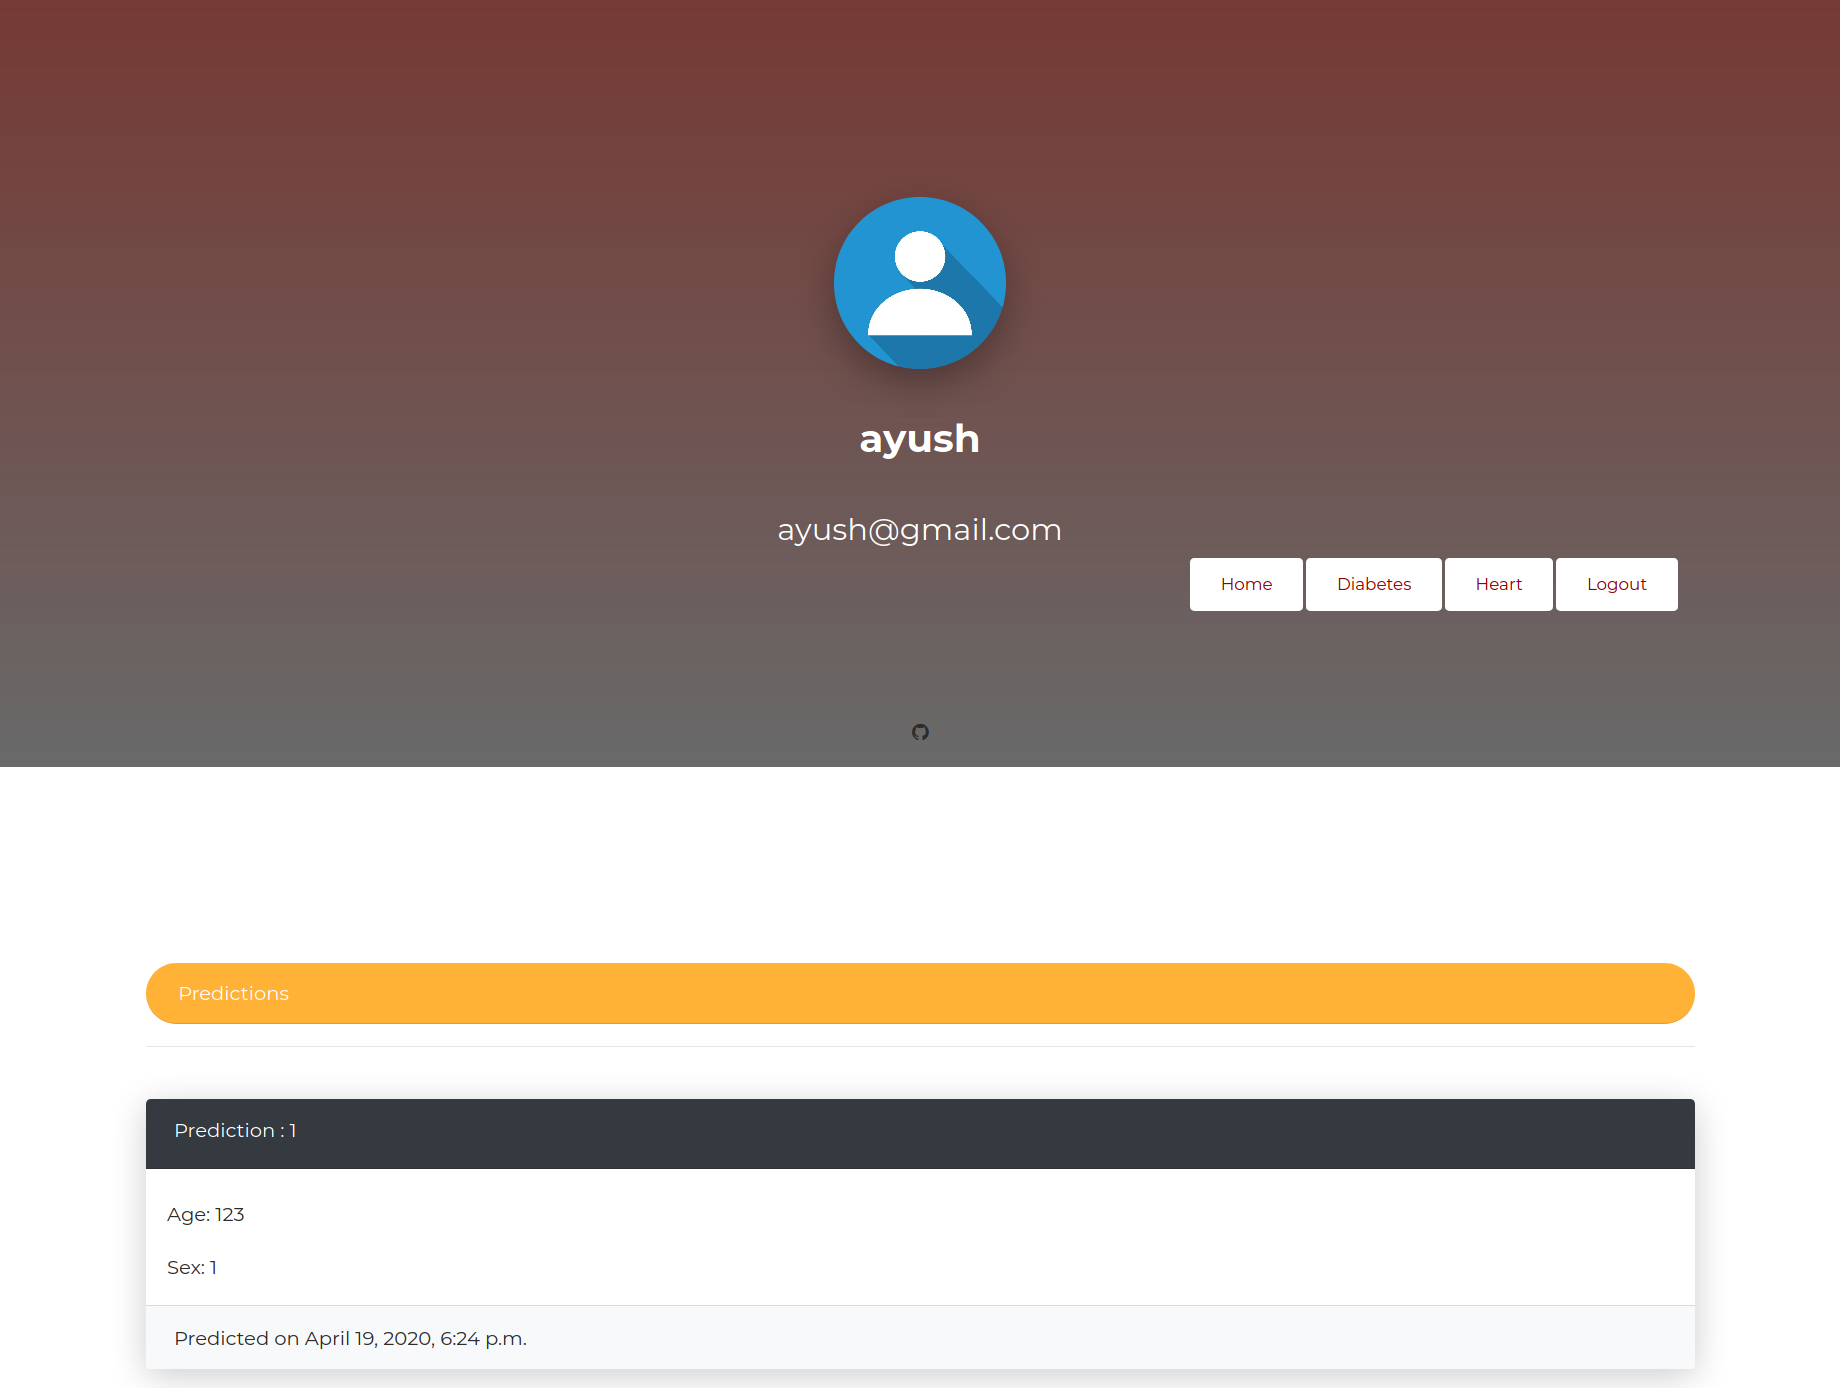
\includegraphics[width=17cm]{Screenshots/profile.PNG}
    				\caption{Profile of a patient showing the past results}
    				\end{center}
    			\end{figure}
    
    \pagebreak
    \section{Data Structures and Algorithms}
    	This section deals with data structure and algorithms we have used in our project.
    	
    \subsection{Naive Bayes Classifier}
    	Naive Bayes classifiers are a group of straightforward probabilistic classifiers based by utilizing Bayes theorem with solid (naive) independence assumptions between the highlights. Naive Bayes classifiers are exceptionally versatile by requiring various parameters direct for the number of highlights or indicators as a variable in a learning issue. It is the least complex and the quickest probabilistic classifier, particularly for the preparation stage.\\
    	Naive Bayes classifier is based on Bayes theorem. This classifier uses conditional independence in which attribute value is independent of the values of other attributes. The Bayes theorem is as follows:
    	Let X= {x1, x2, ......, Xn} be a set of n attributes. In Bayesian, X is considered as evidence and H be some hypothesis means, the data of X belongs to specific class C. We have to determine P (H|X), the probability that the hypothesis H holds given evidence i.e. data sample X. According to Bayes theorem the P (H|X) is expressed as: \\
    	\[P(H|X) = \frac{P(X|H) * P(H)}{P(X)}\].
    	
    	\begin{figure}[h]
    		\begin{center}
    			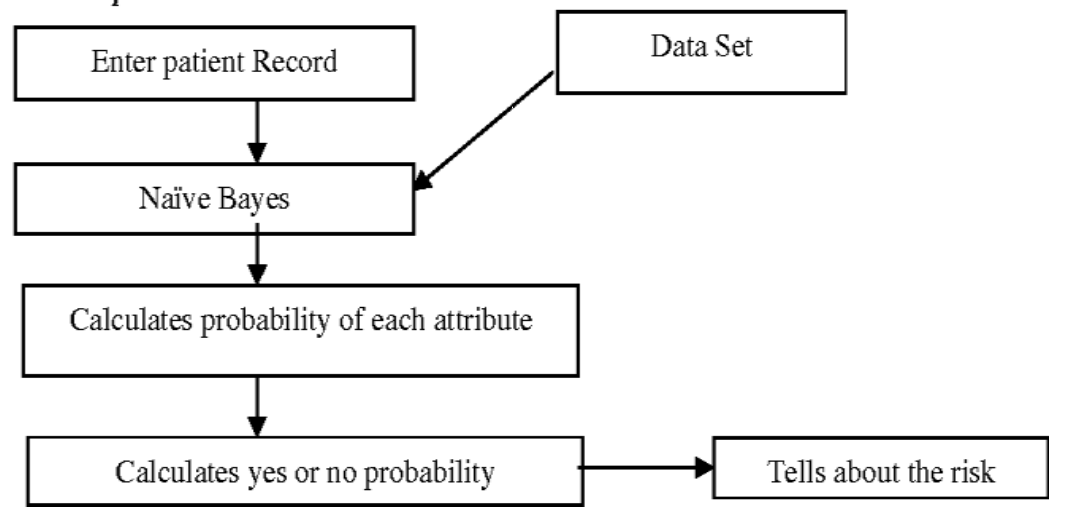
\includegraphics[width = 15cm]{images/naive_bayes.png}\\
    			\caption{Implementation Flow of Naive Bayes Algorithm}
    		\end{center}
    	\end{figure}
    	
       	Utilizing Bayesian classifiers, the framework will find the hidden information related to diseases from authentic records of the patients having heart disease. Bayesian classifiers anticipate the class participation probabilities, such that the likelihood of a given example has a place with a specific class factually. A Bayesian classifier depends on Bayes' theorem. We can utilize Bayes theorem to decide the likelihood that a proposed analysis is right, given the perception. A basic probabilistic, the naive Bayes classifier is utilized for grouping dependent on which depends on Bayes' theorem. As per Naive Bayesian classifier, the event or an event of a specific element of a class is considered as independent in the occurrence or nonoccurrence of some other element. At the point when the element of the sources of info is the high and progressively productive outcome is normal, the boss Naive Bayes Classifier method is appropriate. The Naive Bayes model distinguishes the physical attributes and highlights of patients experiencing heart disease. For each info, it gives the chance of a property of the worthy state. Naive Bayes is a measurable classifier which expects no reliance between properties. This classifier calculation utilizes conditional independence, implies it accept that a quality estimation of a given class is independent of the values of other attributes. The benefit of utilizing Naive Bayes is that one can work with the Naive Bayes model without using any Bayesian methods. (Brownlee, 2016). \\
    	P (Disease|symptom1, symptom2, ..., symptomn) P(Disease)P(symptom1, ..., symptomn|Disease) = P(symptom1, symptom2, ...symptomnN).\\
    	
    	
    
    
    	\subsection{Decision Tree}
    	Decision tree learning utilizes a decision tree as a predictive model which maps perceptions about an item to decisions about the item's target. It is one of the predictive modelling approaches utilized in measurements, information mining and Artificial Intelligence. Tree models where the objective variable can take a finite set of values are called classification trees. In these tree structures, leaves speak to class marks and branches speak to conjunctions of highlights that lead to those class names. Decision trees where the objective variable can take continuous values (ordinarily genuine numbers) are called regression trees. In decision tree analysis, a decision tree can be utilized to outwardly and expressly speak to decisions and decision making. In information mining, a decision tree depicts data but not decisions; rather the subsequent classification tree can be a contribution for decision making.\\
    	The classification tree makes a tree with branches, nodes, and leaves that let us take an unknown data point and descend the tree, applying the traits of the information point to the tree until a leaf is reached and the unknown output of the information point can be determined. To make a decent classification tree model, we have to have a current informational index with known output from which we can build our model. We additionally partition our informational collection into two sections: a training set, which is utilized to build the model, and a test set, which is utilized to check that the model is precise and not overfitted. \\
    	This classifier creates a decision tree based on which it assigns the class values to each data point. Here, we can vary the maximum number of features to be considered while creating the model.\\
    	
    		\begin{figure}
    		\begin{center}
    			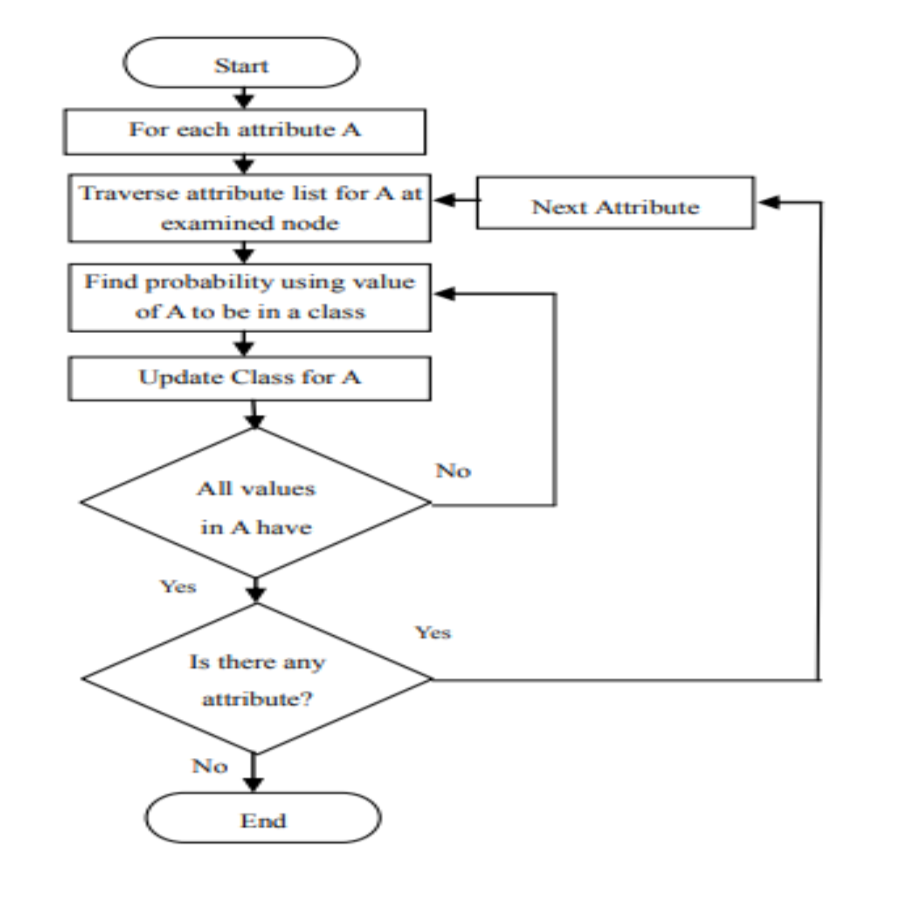
\includegraphics[height=17cm]{images/decision_tree.png}
    			\caption{Flowchart for Decision Tree}
    		\end{center}
    	\end{figure}
    
    	
    	\subsection{Support vector machine(SVM)}
    	SVM was developed by Vladimir Vapnik at AT\&T Bell Labs. It is based on the concept of decision planes that define decision boundaries. A decision plane is a hyperplane that separates the objects having different class memberships. SVM classifiers separate the observations into two or more classes in such a way that maximum separation is achieved. A hypothetical hyperplane is the separator in SVM classification problems.  In other words, SVM constructs a hyperplane that separates the two sets so as to minimize the number of misclassified points. Generally, there are two types of SVM models: linear and nonlinear. Linear SVM works better on linearly separable datasets but nonlinear SVM model works well even on hardly separable datasets. Since we are dealing with hardly separable data in our experiments we use nonlinear SVM. The dual formulation of the nonlinear SVM function can be formulated as
    	\[ MaxW(\alpha) = \sum_{i=1}^{m}\alpha_i - 0.5\sum_{i, j=1}^{m}\alpha_i \alpha_j y_i y_j K(x_i . x_j) \]\\
    	subject to:
    	\[\sum_{i=1}^{m}\alpha_i y_i = 0 ,\]\\
    	\[ 0 \leq \alpha_i \leq C \]\\
    	\begin{figure}
    		\begin{center}
    			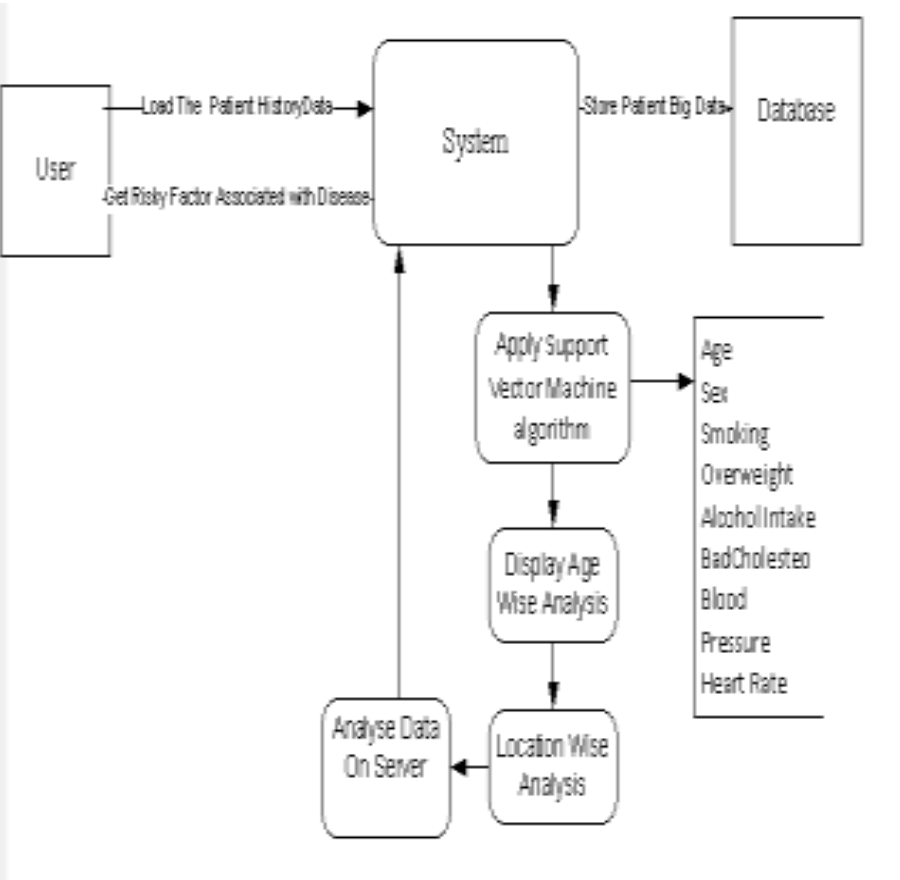
\includegraphics[width=14cm]{images/svm.png}
    			\caption{Flowchart For SVM}
    		\end{center}
    	\end{figure}
    	Input vectors $x_i \in R^m$ , i= 1, 2, 3, …, m, which are called features or attributes are extracted from the database. Associated with every particular input we have a corresponding label ($ y_i = \pm 1$) which is called the target value or output in the database. The variable $\alpha_i$ is the Lagrange multiplier in the dual formulation and C is a user-specified parameter representing the penalty for misclassification K(xi ,xj) is the kernel function and maps the original data points to another space.  One of the popular choices for the kernel is Gaussian kernel which is also known as Radial Basis Function (RBF) in the literature. The formulation for this kernel is
    	\[ K(x_i, x_j) = e^{-\frac{\parallel{x_i - x_j}\parallel^2}{2\sigma}} \]
    	where parameter $\sigma$ is known as the kernel width. 
    	
    	
    	
    	\subsection{Logistic Regression}
    	Logistic Regression is a statistical analysis technique that is used for predicting the data value based on the prior observation of the data set. The logistic regression model predicts the dependent data variable by analyzing the relationship between one or more existing independent variables. Logistic Regression is one of the important tools for prediction, which can also be used for classifying and predicting the data based on the historical data. The implemented model is a binary Logistic model that has dependent variables with only two possible outcomes i.e., one is a positive value and another one is the negative value which is having 0 or 1 as a class label.
    	It mainly consists of two major phases: regularized cost function and regularized gradient descent. Cost Function is used for calculating the maximum likelihood estimation. Gradient descent is an iterative process for getting coefficients from training
    	data. The process is repeated until we get the optimal parameters of train data. The model is trained with the optimal coefficient.Whenever a test data has been passed to the model based on the parameters is able to identify whether the person is having heart disease or not, it tests the data using the sigmoid function. The cost function is the method that is used for reducing the errors of the predicted label and the actual label. Gradient descent function is the method that is used for calculating the coefficient until we obtain a minimum value of the class label.
    	
    		
    	\begin{figure}
    		\begin{center}
    			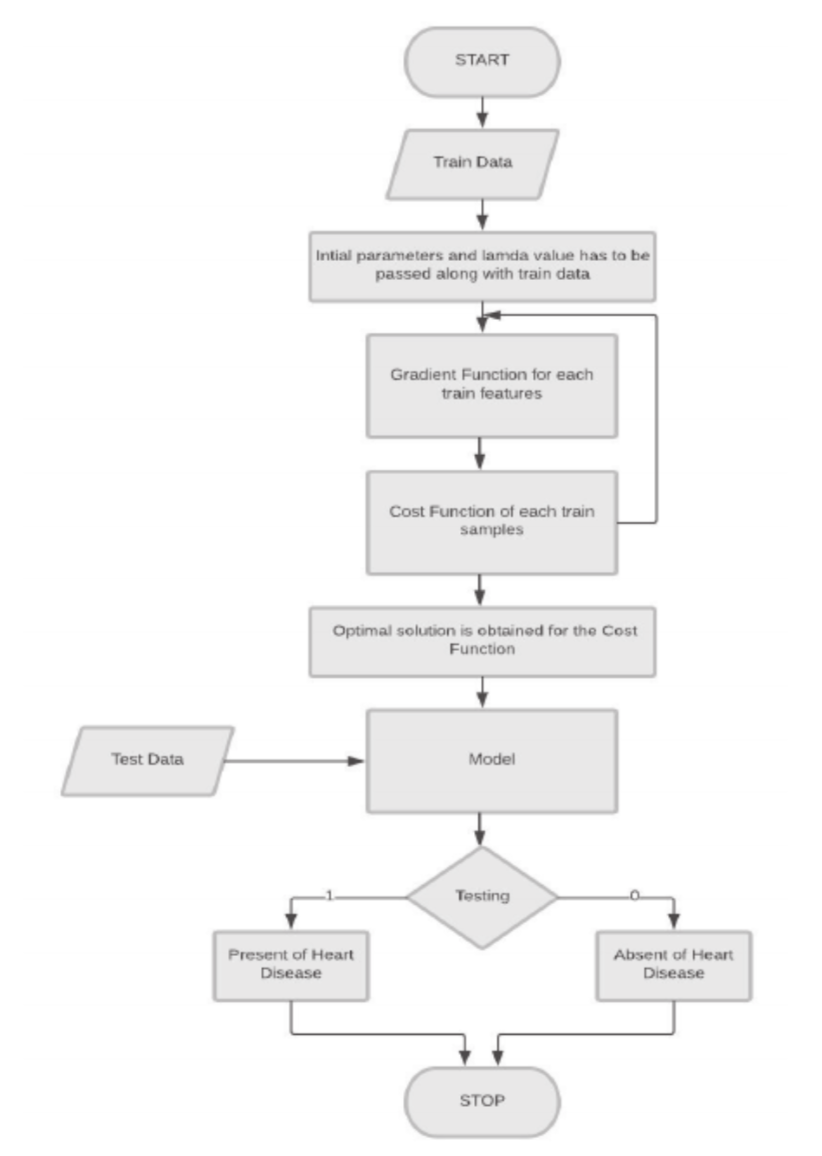
\includegraphics[width=14cm]{images/logistic_regression.png}
    			\caption{FlowChart For Logistic Regression}
    		\end{center}
    	\end{figure}
    	
    	\subsubsection{Cost Function}
    		A minimization function is utilized that is the cost function. It utilizes the Log Loss, for example, the logarithmic loss which quantifies the exhibition of the model where the forecast input esteem is the likelihood between the zero and one. The Log loss is the vulnerability of the forecast which depends on the amount it fluctuates from the real name. Cost function which encourages the learner to address or change the conduct to minimize the errors. The cost function can be assessed by iteratively running the model to look at the predicted value and the known or actual value. The regularized cost function is a technique that is utilized for surviving the danger of overfitting. Lamda is the parameter which controls the regularization term.\\
    		The cost function is calculated by the following:
    		\[ J(\theta) = \frac{1}{m}\sum_{i=1}^{m} y^{(i)} \log[h_\theta(x^{(i)}) - (1-y^{(i)}) \log(1-h_\theta(x^{(i)})] + \frac{\lambda}{2m}\sum_{i=1}^{n}{\theta_j}^2 \] \\
    		m = number of instances \\
    		n = number of attributes \\
    		y = class label \\
    		x = train data features\\
    		$\theta$ = coefficients \\ 
    		$\lambda$ =learning rate
    	
    	
    	\subsubsection{Gradient Descent}
    		Gradient descent is an optimization method which is used to find 
    		the parameters or  the  coefficient  of  the  cost  function.  Gradient 
    		descent is  a  repeated  process  in  order  to  get  the  coefficients  to 
    		minimize the cost function. The  Gradient  descent  is  calculated 
    		for both the classes to get the pair of a coefficient for both class 
    		labels. The goal here is to continue the procedure to try the different 
    		value for the coefficient, evaluating their cost  and selecting the new coefficient that is having the slightly lower cost. Considering this coefficient and storing them in the model. Gradient descent 
    		is calculates as the following:
    		\[ \theta_{ji} = \theta_j - \frac{1}{m}\sum_{i=1}^{m}(h_\theta(x^i)-(y^i)) {x_j}^i + \frac{\lambda}{m} \theta_j \]\\
    		m = number of instances \\
    		x = train data features \\
    		y = class label \\
    		$\theta$ = coefficients \\
    		$\lambda$ = learning rate 
    		
    		
    
    	\subsubsection{Sigmoid Function}
    		Sigmoid function is the logistic function between. This takes the 
    		real input vales and output values between the 0 and 1 for logistic 
    		function [12]. This is interpreted as taking log odds and having 
    		the output probability. Generally sigmoid function is used to map 
    		predictions to probability it is defined as:
    		\[ h_\theta(x) = \frac{1}{1 + e^{-\theta^{T.x}}} \]\\
    		x = test data features \\
    		$\theta$ = coefficients 
    		Whenever a  test  data is passed it calculates  the  value based on 
    		the parameters stored in the model. It calculates the probability 
    		of each class label. We return the maximum probability value of 
    		the class label $x_i$.\\
    		The test data contains the thirteen attributes that we need to pass 
    		and calculate   for both  the classes it will return  the two values 
    		we take the maximum value of two values we will return the class 
    		label which is having the maximum probability.
    	
    	
    	
    		
    		\subsection{K-Nearest Neighbour}  
    		K-Nearest neighbor (KNN) is a simple, lazy and nonparametric classifier. KNN is preferred when all the features are continuous. KNN is also called case-based reasoning and has been used in many applications like pattern recognition, statistical estimation. Classification is obtained by identifying the nearest neighbor to determine the class of an unknown sample. KNN is preferred over other classification algorithms due to its high convergence speed and simplicity.\\
    		KNN classification has two stages
    		\begin{enumerate}
    			\item Find the k number of instances in the dataset that is closest to instance S
    			\item These k number of instances then vote to determine the class of instance S
    		\end{enumerate}
    		The Accuracy of KNN depends on distance metric and K value. Various ways of measuring the distance between two instances are cosine, Euclidean distance. To evaluate the new unknown sample, KNN computes its K nearest neighbors and assign a class by majority voting.\\    		
    		With KNN algorithm, we have chance to change the parameter's weight. It means that, we may assume that some parameters are more important or making more impact than others. Among 8 parameters we use, we can categorize them our data into 2 categories, one is "non-medical" parameters (Age and Sex) and the other is "medical" parameters (CP, Trestbps, Trestbpd etc). We may think that medical parameters are more important than non medical, which we will see in experimental results. Along with weighting, we should find the value of "k" so it gives the best classification result. Since it is a 2-choice classification ("yes") and (“No”) k will be an odd number.
    		
    		\begin{figure}
    			\begin{center}
    				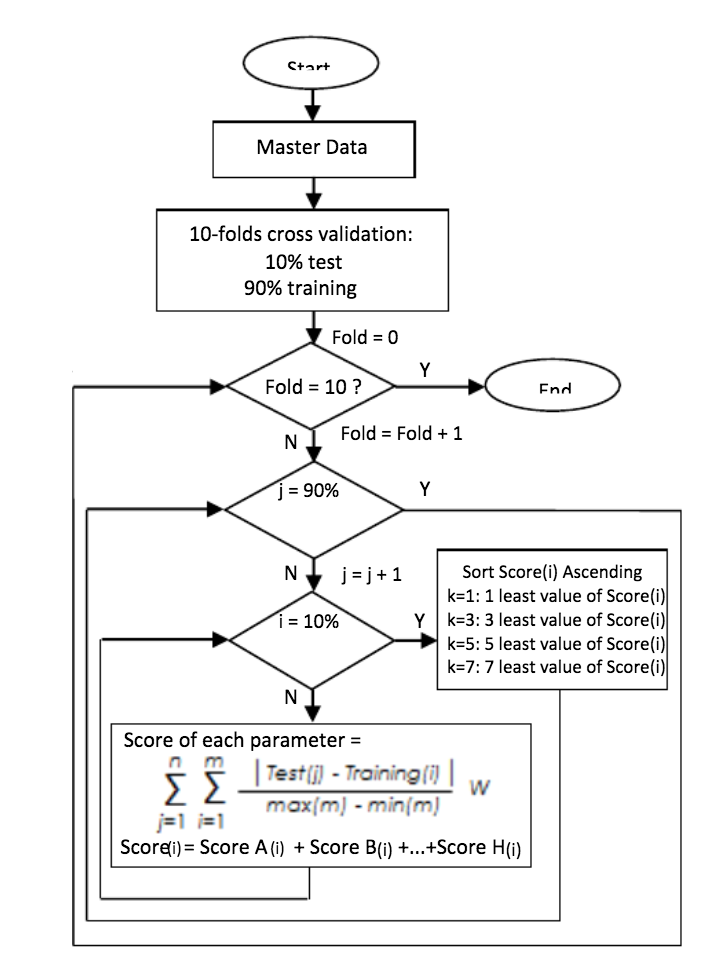
\includegraphics[width=15cm]{images/knn.png}
    				\caption{FlowChart for KNN}
    			\end{center}
    		\end{figure}
    
  		\subsection{Neural Network}
  		\subsubsection{Multilayer Perceptron Neural Network (MLPNN)}
  		One of the most important models in Artificial Neural Network is Multilayer Perceptron
  		(MLP). The  type of architecture  used to  implement  the system  is Multilayer Perceptron Neural Network (MLPNN).
  		\begin{figure}[H]
  			\begin{center}
  				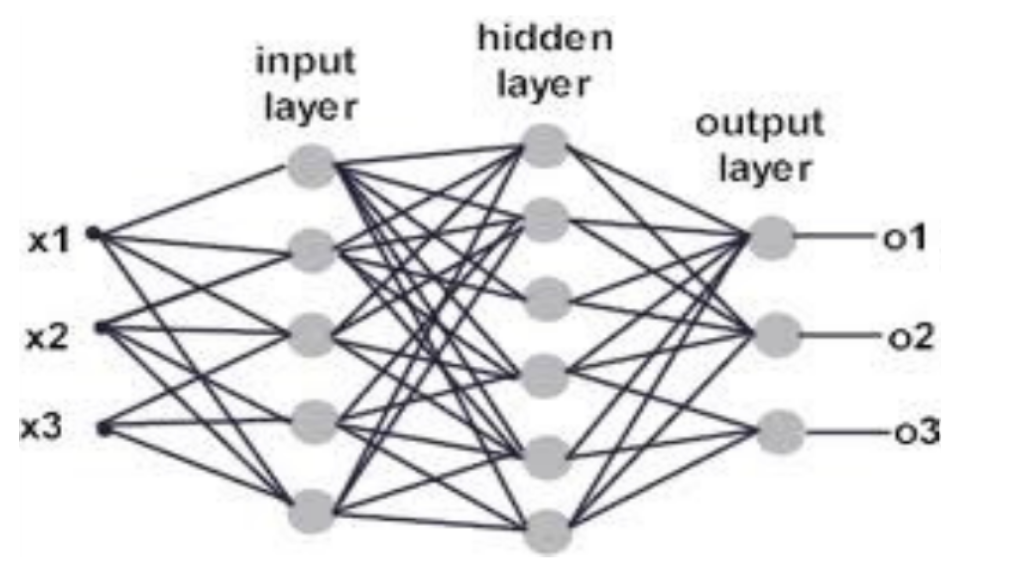
\includegraphics[width=12cm]{images/mlpnn.png}
  				\caption{Neural Network}
  			\end{center}
  		\end{figure}
  		The MLPNN consists of one input layer, one output layer and one or more hidden layers.Each layer consists of one or more nodes, represented by small circles. The lines between nodes indicate flow of information from one node to another node. The input layer receives signals from external nodes. The output of input layer is given to hidden layer, through weighted connection links. It performs computations and transmits the result to output layer through weighted links. The output of hidden layer is forwarded to output layer, it performs computations and produce final result. The working of multilayer perceptron neural network is summarized in steps as mentioned
  		Below:
  		\begin{enumerate}
  			\item Input data  is provided to input layer for processing, which  produces a
  			predicted output.
  			\item The predicted output is subtracted from actual output and error value is
  			calculated.
  			\item  The network then  uses a  Backpropagation algorithm  which  adjusts the
  			weights.
  			\item For weights adjusting it starts from weights between output layer nodes
  			and last hidden layer nodes and works backwards through network.
  			\item When back propagation is finished, the forwarding process starts again.
  			\item The process is repeated until the error between predicted and actual output
  			is minimized.
  		\end{enumerate}
  	\pagebreak
  	
  	\subsubsection{Backpropagation network}
  	The most widely used training algorithm for multilayer and feed forward network is
  	Backpropagation. The name given is back propagation because it calculates the difference between actual and predicted values is propagated from output nodes backwards to nodes in previous layer. This is done to improve weights during processing.The working of Backpropagation algorithm is summarized in steps as follows:
  	\begin{enumerate}
  		\item Provide training data to the network.
  		\item Compare the actual and desired output.
  		\item Calculate the error in each neuron. 
  		\item Calculate what output should be for each neuron and how much lower or
  		higher output must be adjusted for desired output.
  		\item Then adjust the weights
  	\end{enumerate}
  
  \begin{figure}
  	\begin{center}
  			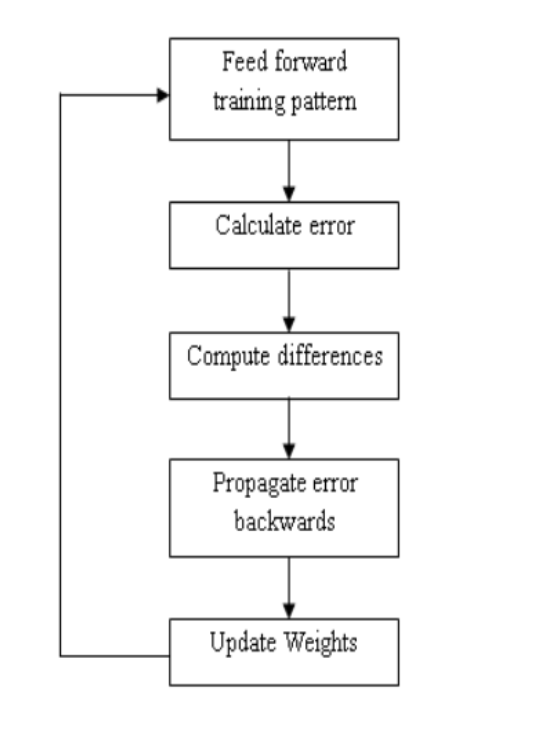
\includegraphics[width=8cm]{images/backpropogation.png}
  			\caption{BackPropagation}
  	\end{center}
  \end{figure}

\begin{figure}[H]
	\begin{center}
		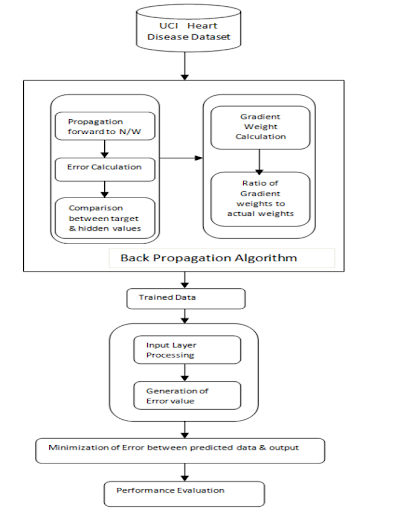
\includegraphics[width=10cm, height=20cm]{images/neural_network.png}
		\caption{Flowchart for Neural Network}	
	\end{center}
\end{figure}

	\section{UML diagrams with discussions} 
	UML is well known for its diagrammatic documentations(Refer Fig 3.10). As a whole 
	realize that UML is for envisioning, indicating, building and recording the segments 
	of programming and non-programming frameworks. Thus, perception is the most 
	critical part which should be comprehended and recollected. UML documentations 
	are the most critical components in demonstrating. Effective and suitable utilization 
	of documentations is imperative for making a total and significant model. The model 
	is pointless, except if its motivation is portrayed legitimately. Consequently, taking 
	in documentations ought to be underlined from the earliest starting point. Diverse 
	documentations are accessible for things and connections. UML graphs are made 
	utilizing the documentations of things and connections. Extensibility is another essential component which makes UML all the more dominant and adaptable. The 
	model’s UML also is quite intuitive and self explanatory, this UML have clear and 
	distinct classes which makes it easily understandable
	\begin{figure}[h]
		\begin{center}
			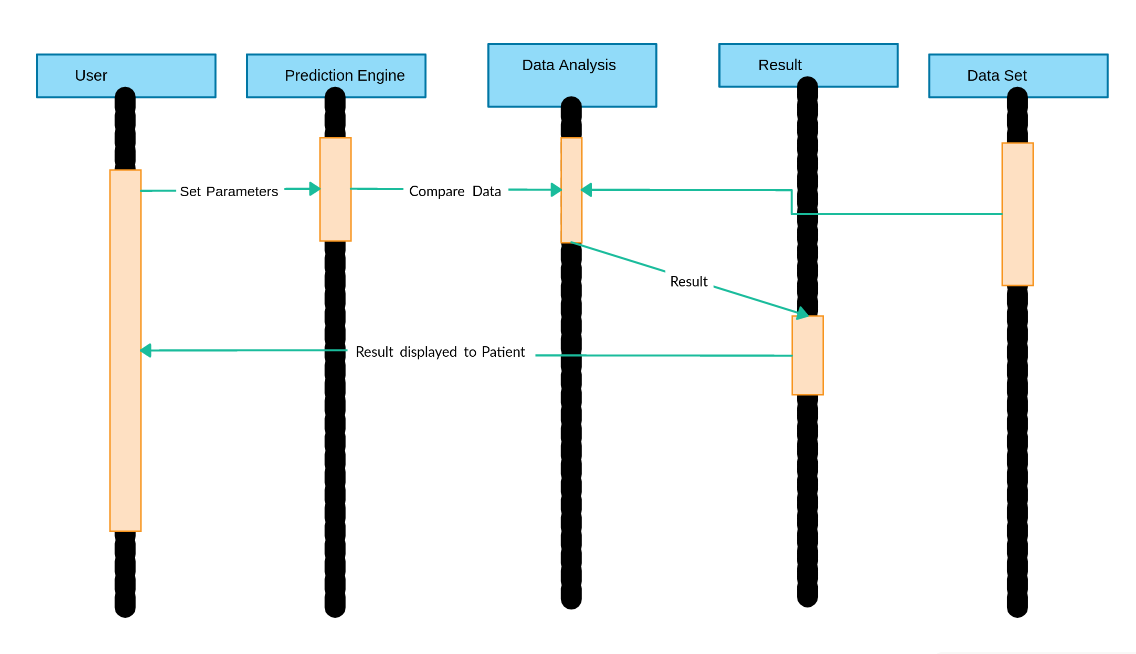
\includegraphics[width=15cm]{images/uml_diagram.png}
			\caption{UML sequence diagram}
		\end{center}
	\end{figure}
	
	
	
	






  	
  	\section{Data Source/Database used and Formats}
  	\subsection{Heart Disease DataSet}
  	The dataset used in this project is the Cleveland Heart Disease dataset taken 
  	from the UCI repository.
  	\begin{center}
  		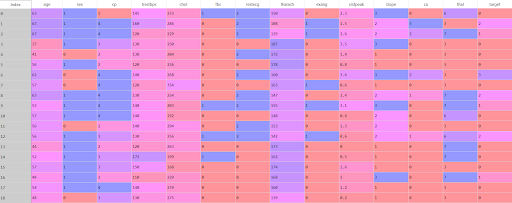
\includegraphics[width=15cm]{images/hdDataset.png}
  	\end{center}
  
  The dataset consists of 303 individuals data. There are 14 columns in the dataset, which    are described below.
  \begin{enumerate}
  	\item\textbf{Age:} displays the age of the individual.
  	
  	\item \textbf{Sex:} displays the gender of the individual using the following format :
  		\begin{itemize}
  			\item 1 = male
  			\item 0 = female
  		\end{itemize}
  	
  	\item \textbf{Chest-pain type:} displays the type of chest-pain experienced by the individual using the following format :
  		\begin{itemize}
  			\item 1 = typical angina
  			\item 2 = atypical angina
  			\item 3 = non — anginal pain
  			\item 4 = asymptotic
  		\end{itemize}
  
  	\item \textbf{Resting Blood Pressure}: displays the resting blood pressure value of an individual in mmHg (unit)
  	
  	\item \textbf{Serum} Cholestrol: displays the serum cholesterol in mg/dl (unit)
  	
  	\item \textbf{Fasting Blood Sugar}: compares the fasting blood sugar value of an individual with 120mg/dl.
  		\begin{itemize}
  			\item If fasting blood sugar > 120mg/dl then, : 1 (true)
  			\item else                                    : 0 (false)
  		\end{itemize}
  	
  	\item \textbf{Resting ECG:} displays resting electrocardiographic results
  	\begin{itemize}
  		\item 0 = normal
  		\item 1 = having ST-T wave abnormality
  		\item 2 = left ventricular hyperthrophy
  	\end{itemize}
  	
  	\item \textbf{Max heart rate achieved:} displays the max heart rate achieved by an individual.
  	\item \textbf{Exercise induced angina} :
	  	\begin{itemize}
  			\item 1 = yes
  			\item 0 = no
  		\end{itemize}
  	
  	\item \textbf{ST depression induced by exercise relative to rest:} displays the value which is an integer or float.
  	
  	\item \textbf{Peak exercise ST segment:}
  		\begin{itemize}
	  		\item 1 = upsloping
  			\item 2 = flat
  			\item 3 = downsloping
 	 	\end{itemize}
  	
  	\item \textbf{Number of major vessels (0–3) colored by flourosopy :} displays the value as integer or float.
  	
  	\item \textbf{Thal :} displays the thalassemia :
  		\begin{itemize}
  			\item 3 = normal
  			\item 6 = fixed defect
  			\item 7 = reversible defect
  		\end{itemize}
  	
  	\item \textbf{Diagnosis of heart disease :} Displays whether the individual is suffering from heart disease or not :
  	\begin{itemize}
  		\item 0 = absent
  		\item 1, 2, 3, 4 = present.
  	\end{itemize}
  	
  \end{enumerate}

	\textbf{Why these parameters:}
	In the actual dataset, we had 76 features but for our study, we chose only the above 14 because :
	
	\begin{enumerate}
		\item \textbf{Age:} Age is the most important risk factor in developing cardiovascular or heart diseases, with approximately a tripling of risk with each decade of life. Coronary fatty streaks can begin to form in adolescence. It is estimated that 82 percent of people who die of coronary heart disease are 65 and older. Simultaneously, the risk of stroke doubles every decade after age 55.
		
		\item \textbf{Sex:} Men are at greater risk of heart disease than pre-menopausal women. Once past menopause, it has been argued that a woman’s risk is similar to a man’s although more recent data from the WHO and UN disputes this. If a female has diabetes, she is more likely to develop heart disease than a male with diabetes.
		Angina (Chest Pain): Angina is chest pain or discomfort caused when your heart muscle doesn’t get enough oxygen-rich blood. It may feel like pressure or squeezing in your chest. The discomfort also can occur in your shoulders, arms, neck, jaw, or back. Angina pain may even feel like indigestion.
	
		\item \textbf{Resting Blood Pressure:} Over time, high blood pressure can damage arteries that feed your heart. High blood pressure that occurs with other conditions, such as obesity, high cholesterol or diabetes, increases your risk even more.
		
		\item \textbf{Serum Cholesterol:} A high level of low-density lipoprotein (LDL) cholesterol (the “bad” cholesterol) is most likely to narrow arteries. A high level of triglycerides, a type of blood fat related to your diet, also ups your risk of a heart attack. However, a high level of high-density lipoprotein (HDL) cholesterol (the “good” cholesterol) lowers your risk of a heart attack.
		
		\item \textbf{Fasting Blood Sugar:} Not producing enough of a hormone secreted by your pancreas (insulin) or not responding to insulin properly causes your body’s blood sugar levels to rise, increasing your risk of a heart attack.
		
		\item \textbf{Resting ECG:} For people at low risk of cardiovascular disease, the USPSTF concludes with moderate certainty that the potential harms of screening with resting or exercise ECG equal or exceed the potential benefits. For people at intermediate to high risk, current evidence is insufficient to assess the balance of benefits and harms of screening.
		
		\item \textbf{Max heart rate achieved:} The increase in cardiovascular risk, associated with the acceleration of heart rate, was comparable to the increase in risk observed with high blood pressure. It has been shown that an increase in heart rate by 10 beats per minute was associated with an increase in the risk of cardiac death by at least 20\%, and this increase in the risk is similar to the one observed with an increase in systolic blood pressure by 10 mm Hg.
		
		\item \textbf{Exercise induced angina:} The pain or discomfort associated with angina usually feels tight, gripping or squeezing, and can vary from mild to severe. Angina is usually felt in the center of your chest but may spread to either or both of your shoulders, or your back, neck, jaw or arm. It can even be felt in your hands. o Types of Angina a. Stable Angina / Angina Pectoris b. Unstable Angina c. Variant (Prinzmetal) Angina d. Microvascular Angina.
		
		\item \textbf{Peak exercise ST segment:} A treadmill ECG stress test is considered abnormal when there is a horizontal or down-sloping ST-segment depression $\geq$ 1 mm at 60–80 ms after the J point. Exercise ECGs with up-sloping ST-segment depressions are typically reported as an ‘equivocal’ test. In general, the occurrence of horizontal or down-sloping ST-segment depression at a lower workload (calculated in METs) or heart rate indicates a worse prognosis and higher likelihood of multi-vessel disease. The duration of ST-segment depression is also important, as prolonged recovery after peak stress is consistent with a positive treadmill ECG stress test. Another finding that is highly indicative of significant CAD is the occurrence of ST-segment elevation > 1 mm (often suggesting transmural ischemia); these patients are frequently referred urgently for coronary angiography.
	\end{enumerate}

	\subsection{Diabetes DataSet}
	The dataset used in this project is the dataset taken from Kaggle which consist of 768 individual data with 8 column variables.\\
	Description of variables in the dataset:
	\begin{enumerate}
		\item \textbf{Pregnancies:} The number of times the given individual has been pregnant.
		\item \textbf{Glucose:} Plasma glucose concentration over 2 hours in an oral glucose tolerance test.
		\item \textbf{BloodPressure:} Diastolic blood pressure (mm Hg).
		\item \textbf{SkinThickness:} Triceps skin fold thickness (mm).
		\item \textbf{Insulin:} 2-Hour serum insulin (mu U/ml).
		\item \textbf{BMI:} Body mass index $(weight in kg)/(height in m)^2$
		\item \textbf{DiabetesPedigreeFunction:} Diabetes pedigree function(a function which scores likelihood of diabetes based on family history).
		\item \textbf{Age:} Age (years).
		\item \textbf{Outcome:} Class variable.
		\begin{itemize}
			\item 0 = absent
			\item 1 = present
		\end{itemize}
		
	\end{enumerate}
	
	\chapter{Implementation}
	\section{Tools and Technologies}
	\subsection{Django}
	Django styles itself as "an elevated level Python web system that supports fast turn of events and perfect, down to business plan. Worked by experienced designers, it deals with a great part of the issue of web improvement, so you can concentrate on composing your application without expecting to waste time." And they truly would not joke about this! This enormous web system accompanies such a significant number of batteries incorporated that as a rule during advancement it very well may be a riddle concerning how everything figures out how to cooperate. Notwithstanding the system itself being enormous, the Django people group is totally gigantic. Actually, it's so enormous and dynamic that there's an entire site dedicated to the outsider bundles individuals have intended to plug into Django to do an entire host of things. This incorporates everything from confirmation and approval, to all out Django-controlled substance the executives frameworks, to web based business additional items, to combinations with Stripe. Discussion about not re-developing the wheel; odds are on the off chance that you need something finished with Django, somebody has just done it and you can simply maneuver it into your venture.
	\subsection{Python}
	Python is a deciphered, significant level, broadly useful programming language. Made by Guido van Rossum and first discharged in 1991, Python's plan theory accentuates code intelligibility with its prominent utilization of huge whitespace. Its language builds and item situated methodology intend to assist software engineers with composing clear, legitimate code for little and enormous scope ventures. 

Python is progressively composed and trash gathered. It bolsters various programming standards, including organized (especially, procedural), object-arranged, and practical programming. Python is regularly portrayed as a "batteries included" language because of its extensive standard library. 

Python was considered in the late 1980s as a replacement to the ABC language. Python 2.0, discharged in 2000, presented highlights like rundown understandings and a trash assortment framework fit for gathering reference cycles. Python 3.0, discharged in 2008, was a significant amendment of the language that isn't totally in reverse good.

	\subsection{SqlLite}
	 SQLite is a little database application that is utilized in a great many programming and gadgets. SQLite was concocted by D.Richard Hipp in August 2000. SQLite is an elite, lightweight social database. In the event that you are happy to get familiar with the internals of a database at a coding level, at that point SQLite is the best open-source database accessible out there with profoundly coherent source code with bunches of documentation. SQLite database engineering split into two unique segments named as center and backend. Center segment contains Interface, Tokenizer, Parser, Code generator, and the virtual machine, which make an execution request for database exchanges. Backend contains B-tree, Pager and OS interface to get to the document framework. Tokenizer, Parser and code generator out and out named as the compiler which creates a lot of opcodes that sudden spikes in demand for a virtual machine.
	
	\subsection{IntelliJ IDEA}
	IntelliJ IDEA is a integrated development environment (IDE) written in Java for creating PC programming. It is created by JetBrains (once in the past known as IntelliJ), and is accessible as an Apache 2 Licensed people group version, and in an exclusive business release. Both can be utilized for business advancement. The IDE gives certain highlights like code fruition by investigating the unique situation, code route which permits bouncing to a class or statement in the code straightforwardly, code refactoring, code troubleshooting , linting and choices to fix irregularities through proposals. The IDE furnishes mix with construct/bundling devices like snort, grove, gradle, and SBT. It bolsters adaptation control frameworks like Git, Mercurial, Perforce, and SVN. Databases like Microsoft SQL Server, Oracle, PostgreSQL, SQLite and MySQL can be gotten to straightforwardly from the IDE in the Ultimate release, through an inserted variant of DataGrip. IntelliJ underpins modules through which one can add extra usefulness to the IDE. Modules can be downloaded and introduced either from IntelliJ's module store site or through the IDE's inbuilt module look and introduce highlight. Every version has separate module storehouses, with both the Community and Ultimate releases totaling more than 3000 modules each starting at 2019..
	
	\subsection{Machine Learning}
	A decent beginning at a Machine Learning definition is that it is a center sub-territory of Artificial Intelligence (AI). ML applications gain for a fact (well information) like people without direct programming. At the point when presented to new information, these applications learn, develop, change, and create without anyone else. As such, with Machine Learning, PCs find savvy data without being advised where to look. Rather, they do this by utilizing calculations that gain from information in an iterative procedure. 

While the idea of Machine Learning has been around for quite a while (think about the WWII Enigma Machine), the capacity to robotize the use of complex scientific estimations to Big Data has been picking up energy in the course of the most recent quite a long while. 

At a significant level, Machine Learning is the capacity to adjust to new information freely and through emphasess. Fundamentally, applications gain from past calculations and exchanges and use "design acknowledgment" to deliver dependable and educated outcomes.
	\subsection{HTML}
	Hypertext Markup Language (HTML) is the standard markup language for archives intended to be displayed in an internet browser. It very well may be helped by advancements, for example, Cascading Style Sheets (CSS) and scripting languages, for example, JavaScript. 

Internet browsers get HTML archives from a web server or from neighborhood stockpiling and render the reports into interactive media website pages. HTML portrays the structure of a website page semantically and initially included signals for the appearance of the report. 

HTML components are the structure squares of HTML pages. With HTML develops, pictures and different articles, for example, intuitive structures might be installed into the rendered page. HTML provides a way to make organized archives by meaning auxiliary semantics for content, for example, headings, paragraphs, records, connections, cites and different things. HTML components are portrayed by labels, composed utilizing point sections. Labels, for example, <img/> and <input/> straightforwardly bring content into the page. Different labels, for example, <p> encompass and provide data about record message and may incorporate different labels as sub-components. Programs don't display the HTML labels, yet use them to interpret the substance of the page.

	\subsection{Cascading Style Sheets}
	Cascading Style Sheets (CSS) is a style sheet language utilized for portraying the introduction of an archive written in a markup language like HTML. CSS is a foundation innovation of the World Wide Web, close by HTML and JavaScript. CSS is intended to empower the partition of introduction and substance, including design, hues, and textual styles. This partition can improve content openness, give greater adaptability and control in the determination of introduction qualities, empower various website pages to share arranging by indicating the significant CSS in a different .css document, and diminish unpredictability and reiteration in the basic substance.
	
	\section{Experimental Setup}
	\begin{enumerate}
		\item 10th Generation Intel® Core™ i7 Processors 8M Cache, up to 3.90 GHz
		\item Disk space 1TB.
		\item Operating System: Linux 18.04. 
	\end{enumerate}
	
	\textbf{Recommended System Requirements}  
	
	\begin{itemize}
		\item Intel® Core™ i5-8257U Processor 6M Cache, up to 3.90 GHz, 8 GB of DRAM. 
		\item Operating systems:  Linux 18.04.
	\end{itemize}
	
	\textbf{Minimum System Requirements}
	
	\begin{enumerate}
		\item Processors: Intel Atom® processor or Intel® Core™ i3 processor.
		\item Disk space: 1 GB 
		\item Operating systems: Windows* 7 or later, macOS, and Linux 
		\item Python* versions: 2.7.X, 3.6.X 
		\item Included development tools: conda*, conda-env, Jupyter Notebook* (IPython) 
		\item Compatible tools: Microsoft Visual Studio*, PyCharm*Included Python packages - NumPy, SciPy, scikit-learn*, pandas, Matplotlib, Numba*, Intel® Threading Building Blocks, pyDAAL, Jupyter, mpi4py, PIP*, and other 
	\end{enumerate}
	\section{Coding Standards followed}
	When it comes to the coding styles or coding standards, Developers have wide range of flexibility, on the basis of several parameters, be it any design. A good designed code as that in the current project takes into account the following:
	\begin{itemize}
		\item prper documentation has been done by comments
		\item caode is been refactored and extra spaces has been removed 
		\item proper libary has been imported
		\item proper message hass been added while commiting the code 
		\item proper naming conventions has been followed
		\item meaningful variable names has been used
		\item OOP concept has been used 
		\item Code is written in a genral for proper re-usabilty 
	\end{itemize}
	
	\section{Code Integration details}
	The code integration has been done using GIT as the version control. The python code has been well packed in modules which has provided ease of integration. The HTML forms are provided by means of python class by creating object for each input entity and adding constraints to those classes which makes the HTML page dynamic and easy to adapt new changes. The project is designed in such a way that files names and location are specified through regex. The modules are enclosed in packages which increase the readability and simplicity of code. The machine learning algorithms uses a file to read new data provided by user and to predict the result. This prediction result is passed to the prediction page through a data provider class. The prediction data is stored in database for keeping track of predictions.
	
	\section{Implementation work flow}
	Implementation takes into account type of algorithm used in the project, its efficiency, so that the use of the most possible efficient algorithm can be used, based on the use case, design and the development team. This project has been built over similar definition of implementation, wherein each aspect of implementation has been taken care of, right from the design of the UI to database, algorithms to api . A particular design pattern has been followed to promote scalability and proper maintenance of the code. The work flow starts right from the design implementation and ends on code implementation. Algorithm has been used which calculates the possibility of diseases based on the details provided by the patient. Authentication and validation of user data has been taken into account and all the history of searches made are stored in the database with timestamp.
	\subsection{Data cleaning}
	data cleaning tasks using Python’s Pandas library. Specifically, we’ve focus on probably the biggest data cleaning task, missing values.
	\subsubsection{Sources of Missing Values}
	\begin{itemize}
		\item User forgot to fill in a field.
		\item Data was lost while transferring manually from a legacy database.
		\item There was a programming error.
		\item Users chose not to fill out a field tied to their beliefs about how the results would be used or interpreted. 
	\end{itemize}
	If we take a look at the coloums of dataset,we can see that Pandas filled in the blank space with “NA”. Using the isnull() method, we can confirm that both the missing value and “NA” were recognized as missing values. Both boolean responses are True. Pandas will recognize both empty cells and “NA” types as missing values.But there are values of some types that Pandas won’t recognize.
	\subsubsection{Non-Standard Missing Values}
	If there’s multiple users manually entering data, then this is a common problem. Maybe some like to use “n/a” but other like to use “na”. An easy way to detect these various formats is to put them in a list. Then when we import the data, Pandas will recognize them right away.below is the example of how its done here.
	\begin{figure}
  	\begin{center}
  			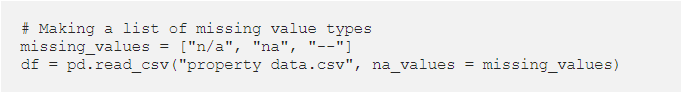
\includegraphics[width=8cm]{images/datacleaning.png}
  			\caption{making a list of missing values}
  	\end{center}
  \end{figure}
  
  \subsection{Handling unstructured and structured Data} Python supports good libraries for handling structured and unstructured data
  \begin{itemize}
		\item \textbf{Python processing CSV data}
		\begin{itemize}
		\item The csv file is a text file in which the values in the columns are separated by a comma. Let's consider the following data present in the file named input.csv.
		\item we can create this file using windows notepad by copying and pasting this data. Save the file as input.csv 
				\item The read csv function of the pandas library is used read the content of a CSV file into the python environment as a pandas DataFrame. The function can read the files from the OS by using proper path to the file.
		\item The read csv function of the pandas library can also be used to read some specific rows for a given column.
		\end{itemize} 
		\item \textbf{Python processing JSON data}
			\begin{itemize}
		\item Create a JSON file by copying the below data into a text editor like notepad. Save the file with .json extension
		\item The read json function of the pandas library can be used to read the JSON file into a pandas DataFrame. 
		\item  the read json function of the pandas library can also be used to read some specific columns and specific rows after the JSON file is read to a DataFrame. We use the multi-axes indexing method called .loc $($ $)$ for this purpose.
		\item We can also apply the tojson function along with parameters to read the JSON file content into individual records.
		\end{itemize} 
	\end{itemize}
  
	\section{Execution Results and Discussions}
	The results of execution of the code are quite satisfactory. A complete flow of the application can be observed, without any fatal error and code break. Some of the
instances are as follows:
	\begin{itemize}
		\item User should be able to signup with email and password
		\item Existing user should be able to login with valid email and pasword of more the length of 6 characters
		\item User should be able to predict the heart disease 
		\item User should be able to predict the diabetes  
		\item User should be able to move to the contact page of development team by clicking on contact button 
		\item User should be able to logout from its account succesfully 
		
	\end{itemize}
	\section{Non-functional requirements results}
	\begin{enumerate}
		\item \textbf{Performance parameters} This includes the response time of the system utilization level of both static and volumetric type throughput etc. these parameters are standardized so a system has to follow them
		\item \textbf{Corrective Maintenance} In case of any bugs left in the system, the bugs and issues will be fixed for smooth running of application. The accuracy of the system can be further improved with other algorithm if needed
		\item \textbf{Adaptive maintenance} The features in the applications can be added sauch as history of the disease can be kept in the log. the available list of symptoms can also be added for covering more number of diseases.
		\item \textbf{Security} Amazon web services uses several operational security features like vulnerability management, malware prevention, monitoring, incident management, server and software stack security, trusted server boot, secured service APIs and authenticated access, data encryption, network firewall rule maintenance. 
		\item \textbf{Interoperability} This requirement demands the system to be built in such a way that it can work in integration with different operating systems and can be changed as per the user requirements.Since the end product of this project is a web app hosted on AWS cloud, therefore the web app can be accessed by any user on any device through the internet. 
	\end{enumerate}
	
	
	\chapter{Testing}
	
	\section{Test workflow}
	\subsection{Integration Testing}
	Testing with respect to integration of components of the application. This type of testing is done after the application is wholly developed, in order to check the integration with all the boundary cases considered. An app is said to pass the integration testing only when all the components are integrated to each other with a full fledged flow, and the code does not break across any module or component. This testing is done generally through automation as a manual testing with respect to integrationwould not test the same on multiple parameters based on real time data.

	\subsection{Unit based Testing}
	This kind of testing manages testing of each class/strategy/business rationale as a unit. Unit testing is one of the fabulous techniques for testing which advances free coupling as each bit of utilization case as a business rationale is kept up as a nuclear unit. No two techniques have same usefulness. Notwithstanding that a technique is structured distinctly to deal with one use case. The strategies just holds business rationale decoupled from any instrument parts, explicitly android for our situation. In the application, MVP configuration design has been utilized which is the most capable plan design with regards to unit testing. This engineering has been utilized on the grounds that it makes the business rationale liberated from the android parts and makes it simpler to perform unit testing with no coupling. All the system calls have been done in the moderator layer, wherein the view layer is obscure of the system calls and related information. The moderator is put to test as and when required.
	
	\subsection{Validation Testing}
	It starts at the completion of coordination testing, when specific parts have been worked out, the thing is totally gathered as a bundle, and interfacing bungles have been revealed and rectfied. At the endorsement or structure level, the capability between traditional programming, fight arrangedprogramming, and WebApps disappears. The way toward studying programming amidst the change framework or toward the total of the progress technique to pick if it fulfills chose business necessities. It guarantees that the thing genuinely addresses the customer's issues. It can in like way be depicted as to exhibit that the thing satisfies its ordinary use when sent on sensible condition. It addresses the inquiry, Are we making the correct thing?
	
		\section{Test case details}
	\subsection{Test case 1:}
	Unit to test: User Authentication\\
	Assumptions:\\
	\begin{itemize}
		\item A Patient is a first time user
		\item A Patient can also be an existing user
		\item He enters a correct password which belongs to him
	\end{itemize}
	Test data: minimum six digit passwors\\
	\\
	Steps to be executed:
	\begin{itemize}
		\item A first time user enters his username, email, password, confirm password
		\item Following the above clicks on submit button
		\item Moves to to the home page of the application
	\end{itemize}
	Expected result:
	\begin{itemize}
		\item user should be redirected to the home page where he gets option to predict heart or diabetes disease
	\end{itemize}
	Actual result:when user enters first time and signUp with email and password, he shoud be redirected to the home page\\
	\\
	Pass/Fail: Passed\\
	\\
	Comments:  The test was successful, everything worked fine
	
	\subsection{Test case 2:}
	Unit to test: verification of home page details\\
	Assumptions:\\
	\begin{itemize}
		\item A Patient is a first time user
		\item A Patient can also be an existing user
		\item He enters a correct password which belongs to him
	\end{itemize}
	Test data: user should have login with correct username and password\\
	\\
	Steps to be executed:\\
	\begin{itemize}
		\item Home page should have buttons for heart diseases prediction and diabetes prediction
		\item it sgould also contains all the navigable buttons in th top corners of website
		\item Moves to to the corresponding page of the application when click on any button.
	\end{itemize}
	Expected result:  Moves to to the corresponding page of the application when click on any button.\\
	\\
	Actual result: user should be able to navigate throughout the website\\
	\\
	Pass/Fail: Passed\\
	\\
	
	\subsection{Test case 3:}
	Unit to test: database storage of patients\\
	Assumptions:\\
	\begin{itemize}
		\item Admin user name and password.
	\end{itemize}
	Test data: Admin should have login with correct username and password\\
	\\
	Steps to be executed:\\
	\begin{itemize}
		\item Admin login button should be clicked
		\item admin should enter correct login details in django administrator
		\item admin should see all the patients results and the user accounts registered
	\end{itemize}
	Expected result:  admin should see all the patients results and the user accounts registered\\
	\\
	Actual result: Admin should be able to see all the records for patients\\
	\\
	Pass/Fail: Passed\\
	\\
	Comments: The test was successful, everything worked fine
	
	\subsection{Test case 4:}
	Unit to test: working of prediction engine for Heart diseases \\
	Assumptions:\\
	\begin{itemize}
		\item Home page should have buttons for heart diseases prediction and diabetes prediction
		\item it should also contains all the navigable buttons in th top corners of website
		\item Moves to to the corresponding page of the application when click on any button.
	\end{itemize}
	Test data: patient report details\\
	\\
	Steps to be executed:\\
	\begin{itemize}
		\item user should click on predict heart disease button
		\item user should enter all the details in the form for heart diseases prediction engine
		\item user should click on predict button
	\end{itemize}
	Expected result:  user should be able to see the possibility of heart disease by various algorithms used to predict\\
	\\
	Actual result: result should be displayed by different algorithm\\
	\\
	Pass/Fail: Passed\\
	\\
	Comments: The test was successful, everything worked fine
	
	\subsection{Test case 5:}
	Unit to test: working of prediction engine for diabetes diseases \\
	Assumptions:\\
	\begin{itemize}
		\item Home page should have buttons for heart diseases prediction and diabetes prediction
		\item it should also contains all the navigable buttons in th top corners of website
		\item Moves to to the corresponding page of the application when click on any button.
	\end{itemize}
	Test data: patient report details\\
	\\
	Steps to be executed:\\
	\begin{itemize}
		\item user should click on predict diabetes button
		\item user should enter all the details in the form for diabetes prediction engine
		\item user should click on predict button
	\end{itemize}
	Expected result:  user should be able to see the possibility of diabetes by various algorithms used to predict\\
	\\
	Actual result: result should be displayed by different algorithm\\
	\\
	Pass/Fail: Passed\\
	\\
	Comments: The test was successful, everything worked fine
	
	
	\def\baselinestretch{1}
	\chapter{Conclusions and Future Scope}
	\def\baselinestretch{1.66}

	\paragraph{} This project uses the various machine learning algorithms such as support vector machine, NaïveBayes,   decision   tree,  k-nearest neighbour, neural network, logistic regression which were applied  to  the data   set.  It  utilizes the data such  as blood  pressure, cholesterol,  diabetes etc and then tries to predict the possibility of heart disease. Family history of heart disease can also be a reason for developing a heart disease as mentioned earlier.This work will be useful in identifying the possible patients who may  suffer from heart disease in the next 10 years. The most efficient algorithm was to be selected based on various criteria. The accuracies found by different algorithims are as follow :-\\
	\begin{itemize}
		\item support vector machine   0.8289   
		\item  NaïveBayes   0.8000   
		\item decision tree   0.8043
		\item  k-nearest neighbour   0.8913 
		\item neural network   0.9700 
		\item logistic regression 0.8500\\
	\end{itemize}
	We found out that the neural network algorithm was the most efficient out of the three with an accuracy of 97 percentage. Thus the logistic regression algorithm was further implemented using different applications. For this, jupiter notebook was used. Since heart diseases are major killer in India and throughout the world, the application of a promising technology like machine learning to the initial prediction of heart diseases will have a profound impact on society. There are numerous conceivable enhancements that could be investigated to improve the adaptability and exactness of this predicted system. By training the model with different dataset may lead to best fit model because this heart disease data set may vary with years. It could be more benefited by changing the data set and by implementing different algorithms for the prediction of heart disease may increase the efficiency of the prediction.\\
	\\
	 This may help in taking preventivemeasures and hence try to avoid the possibility ofheart disease for the patient. So when a patient ispredicted  as  positive  for  heart  disease,  then  themedical data for the patient can be closely analysedby the doctors. An example would be - suppose thepatient  has  diabetes  which may  be  the cause   forheart disease in future and  then the patient can begiven treatment to have diabetes in control which inturn may prevent the heart disease.The  heart  disease  prediction  can  be   done  usin gother   machine   learning   algorithms. Logistic regression can also perform well in case of binary classification   problems   such   as   heart   disease prediction. Random forests can  perform well than decision  trees.   Also, the  ensemble  methods   and artificial neural networks can be applied to the dataset. The results can be compared and improvised
	
	\chapter*{Appendix-A}
	\section*{Pseudocode} 
	
	\begin{itemize}
		\item \textbf{Dividing data into train and test data} The data is divided into 10 fold out of which 9 folds are used to train the data and 1 fold is for testing.
		\item \textbf{HTML Forms} To provide signup detils a form.py class is used which consist of objects for each entity\\
class UserForm(forms.ModelForm): \\
	username $=$ forms.CharField $($ widget $=$ forms.TextInput $($ \\
	attrs $=$ $[$'class': 'form-control', 'placeholder': 'Enter username'$]$ \\
	$)$, required $=$ True, maxlength $=$ 50 $)$ \\
	
	email $=$ forms.CharField $($ widget $=$ forms.EmailInput(  \\
attrs $=$ $[$ 'class': 'form-control', 'placeholder': 'Enter Email Id' $]$  \\
 $)$ , required $=$ True, maxlength $=$ 50 $)$  \\

password $=$ forms.CharField(widget $=$ forms.PasswordInput $($  \\
attrs $=$ $[$ 'class': 'form-control', 'placeholder': 'Enter password' $]$  \\
 $)$ , required $=$ True, minlength $=$ 6, maxlength $=$ 50 $)$  \\

confirmpassword $=$ forms.CharField $($ widget $=$ forms.PasswordInput $($  \\
attrs $=$ $[$ 'class': 'form-control', 'placeholder': 'Confirmpassword' $]$  \\
 $)$, required $=$ True, minlength $=$ 6, maxlength $=$ 50 $)$  \\
 \\
 	\item \textbf{Executing Machine learning models} The prediction results of each machine learning model is stored in a file with the regex expression\\
 	\\
	predictions $=$ $[$ \\
'SVC': str $($ SVCClassifier.predict$($features$)$ $[$0$]$ $)$, \\
'LogisticRegression': str $($ LogisticRegressionClassifier.predict$($features$)$ $[$0$]$ $)$, \\
'NaiveBayes': str $($ NaiveBayesClassifier.predict$($features$)$ $[$0$]$ $)$, \\
'DecisionTree': str $($ DecisionTreeClassifier.predict$($features$)$ $[$0$]$ $)$, \\
'KNN': str $($ KNeighborsClassifier.predict$($features$)$ $[$0$]$ $)$, \\
 'NeuralNetwork': str $($ NeuralNetworkClassifier.predic$($features$)$ $[$0$]$ $)$, $]$ \\
\\
The string NaiveBayesClassifier will look for file naivebaiyes.py and execute it to generate naivebaiyes.pkl $($ executable file$)$

	\item \textbf{Dataprovider.py} It consist of class 
	
	GetAllClassifiersForHeart $($ $)$ : \\
return $($ GetSVCClassifierForHeart $($ $)$, \\
GetLogisticRegressionClassifierForHeart $($ $)$, \\
GetNaiveBayesClassifierForHeart $($ $)$, \\
GetDecisionTreeClassifierForHeart $($ $)$, \\
GetKNeighborsClassifierForHeart $($ $)$, \\
GetNeuralNetworkClassifierForHeart $($ $)$ $)$ \\
\\
Which takes the prediction result from machine learning pkl file and provide it to HTML file to display the result.
	\end{itemize}
	
%\bibliographystyle{plain}
%\cleardoublepage
%\addcontentsline{toc}{chapter}{Bibliography}
\chapter*{Bibliography}
\begin{itemize}
		\item https://www.tutorialspoint.com/pythondatascience/   
		\item  https://towardsdatascience.com/data-cleaning-with-python-and-pandas-detecting-missing-values
		\item Prediction of Heart Disease Using Machine Learning Algorithms  by Rajesh N, T Maneesha, Shaik Hafeez, Hari Krishna 
		\item  A Review on Heart Disease Prediction using Machine Learning and Data Analytics Approach By M. Marimuthu, M. Abinaya , K. S. Hariesh .
		\item https://bmcmedinformdecismak.biomedcentral.com/articles/ 
		\item https://www.kdnuggets.com/2015/12/machine-learning-data-science-apis.html
	\end{itemize}
%\bibliography{References/references}
\end{document}


